\documentclass{ctexbook}

% QCC book needs
\usepackage{fix-cm}  % this package allows large \fontsize
\usepackage{imakeidx}
\makeindex[title=Index]
\usepackage{listings}
\usepackage[table]{xcolor}

\usepackage{amsmath,graphicx}

\usepackage{tikz}    % this is for graphics. e.g. rectangle on title 
\usetikzlibrary{quantikz, decorations.pathmorphing,shapes.geometric}
%\usepackage{circuitikz}
\usepackage{tikz-3dplot} % includes tikz
\tdplotsetmaincoords{70}{120}
\usepackage{float}


% This file is for commands / macros / functions.
% QCC book specific
\newcommand{\keta}[2][]{\vert {#2} \rangle_{#1}}
\newcommand{\braketa}[3][]{\langle {#2} \vert {#3}\rangle_{#1}}

\tikzstyle{Gate}=[rectangle, minimum width=30, minimum height=30, text width=20, text centered, draw=black]
% Content Starts Here
%%\chapter{About the Author}
Yuan John Jiang
\begin{document}
\thispagestyle{empty}

\vspace{3cm}
  \begin{center}
	\bfseries \Huge 不须纠缠的量子信息 \par   %  \latex Your own title would go here.
        ~\\
	\bfseries \LARGE 量子算法和通信协议 \\   % Include a subtitle or just delete.
        ~\\
        \bfseries \Large 江源,邢晓乔,孟璞辉 \par   % The author's name goes here.

        \vspace{3cm}
    
%      	{\centering \includegraphics[width=0.8\linewidth]{images/cover.png}}
    \end{center}
    
\par

\newpage


% The asterisk excludes the chapter from the table of contents.
%\addcontentsline{toc}{chapter}{}
%\chapter*{前言}
%量子计算和通信都是热门技术,但是掌握这些技术的工程师前言包括程序员呢?量子太高深神秘了,加上信息,还闹出爱因斯坦等人提出的量子信息能否超音速传递的EPR悖论。由物理学家主导的量子信息学太难学了。

% Three-level Table of Contents
\setcounter{tocdepth}{3}
\tableofcontents

\mainmatter

\chapter{综述}\label{c-intro}
我们处在一个信息爆炸的世界,这几年蹿红的AI既需要大量信息供它学习,同时,它又制造出更多新的信息加剧了信息爆炸。信息处理的算力远远不够,AI公司更是把算力最强的GPU芯片都买空了,英伟达股票不断飙涨。幸好我们看到了曙光,比GPU算力更强的QPU-量子处理器或量子计算机-会于2030年代进入市场,只争朝夕的硬件工程师们发出了这样的预告。

硬件在飞速发展,那软件呢?懂得量子算法的软件工程师们在哪里?现在的量子信息教程太难懂了,即使博士毕业也不一定能设计量子算法和通信协议。这本书是从全新的思路讲述量子信息,目标是教信息工程相关专业的本科生学会现有的量子算法和通信协议进而能够编程。我们更高的期望是通过这本书的启发,有能力的学生可以进而开展新的算法和协议设计。

量子信息是关于量子波承载,传输和处理信息的理论。一个量子波就是一个量子比特。量子这个词总会让人想起那个神秘的薛定谔猫及各种摸棱两可和不可思议,这就是目前量子信息书的问题。再者这些书不是建立在信息论基础上,很多物理学家甚至否认香农创立的信息论适用于量子信息,用型似的冯纽曼熵替代香农信息熵,试图弥补缺失的信息学基础知识。这样堆砌的量子信息必定艰涩难懂。

本书用新思路讲解量子信息,首先它以信息论为基础,另外,它借助通信理论的框架甚至术语。现代通信用电磁波承载和传输信息,我们每天都用,通信理论是一套非常系统成熟实用的理论。只有从信息论和通信理论延伸的量子信息理论才会系统实用。本书的读者对象是对计算机和通信等基本信息技术有初步了解,并且学过向量和矩阵基本课程的大学生。学过调制和解调等通信技术的学生会很容易进一步学习本书的课题,对于其他学生,第二章补充这方面的基本知识。

\section{信息学}
\subsection{什么是信息?}
信息时常看不见摸不着,好像是个难定义的东西,但在脑子之外,信息总是由纸,声音,电波等介质中的各种符号呈现的。信息是符号,即使在脑子里,神经科学家也指出它是以电信号呈现的。另外信息必须是有用的符号,没用的不是。

当我们在诊所量血压,那个护士会读出我们的血压是多少毫米。我们的生命生理信息怎么能用毫米衡量呢?那是因为不久之前,护士会看一个水银柱高度读出我们的血压值。那就是说信息可以用数字代表,并由水银柱的高度这样的介质的物理量承载或显示。把信息用数字代表,信息学里叫编码(encoding)。现代信息技术都是用数字代表信息的,即使文字可以用写在纸上的字承载和显示,但在电子信息技术里也必须用8位(二进制)的ASCII或更多位的Unicode码代表。所以本书针对的是用数字代表的信息。

\subsection{信息技术三层面}
一个老旧血压计最主要元件是它的玻璃水银柱, 人的血管压力会将水银推到一个高度。水银柱是信息载体同时也是读取显示元件,高度是信息承载参量。代表信息的数字,码或符号总是要用某种介质的物理量承载的。代表信息的数字也叫码(code),通信教课书里也叫符号(symbol)。从血压计的原理,我们看到信息技术有三个层面:信息,数字符号和载体物理量,如图-\ref{fig:3levels}所示。

\begin{figure}\label{fig:3levels}
    \centering
    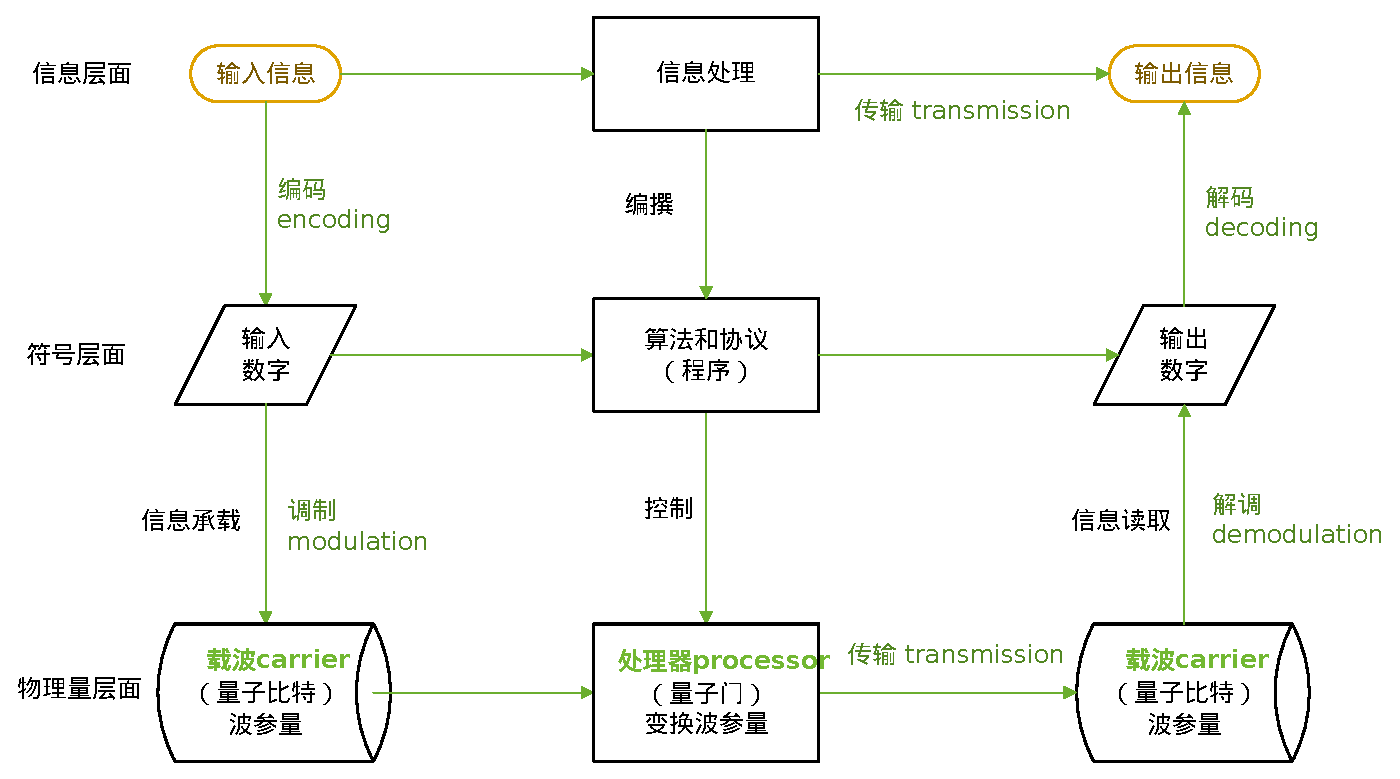
\includegraphics[width=6cm]{pic/qinfo_flow.eps}
    \caption{量子技术三层面}
\end{figure}

抽离承载介质,抽象的信息层面看不见摸不着,但(Claude Shannon, 1916-2001)发展的信息论深刻阐明了信息和数字符号层面的对应关系,让我们以数字符号层面为起点定义和研究信息。所以量子信息学可以集中在数字符号与物理量层面,而不需涉及抽象的信息层面。

香农出身于美国密持根州一个普通家庭,他大部分贡献是在贝尔实验室研究通信理论的成果,是当之无愧的信息论之父。以信息论为基础,通信理论建立了系统完整的符号层面与载体层面的对应关系。通信理论多是贝尔实验室研究成果,但很难说是某一个人的理论。图-\ref{fig:3levels}中所有用蓝色字体的,都是通信名词。怎么用波承载信息,或者说怎么选择波参量与信息数字对应,是通信理论中的调制理论的专题。现代通信都是用电磁波承载和传送信息,量子技术用量子波承载信息,承载信息的物理量不同,两者原理是完全相同的。

一个波的参量可以对应的数字越多,它可承载的信息越多。理论上量子比特可以承载无限多信息,这是量子算力强大所在,图-\ref{fig:3levels}中完成信息处理的量子门电路对波参量实行U变换(unitary transformation,又称酉变换),理论上讲可以实现任何的算法,也就是说实现通用计算机。但是量子比特读取不同于普通通信设备的解调,不是调制的逆过程,能读取出的信息最多是一个比特,这就是我们后面需要不断加深理解的量子比特读取瓶颈。

\subsection{误差限制}
血压计用水银柱高度这个物理量,现代Wi-Fi和手机(5G)通信都用无线电波的波参数,量子比特用量子波的波参数。可是如果我们读出血压为120.5毫米时,这个数字准确吗?倾斜的水银柱会产生系统误差,我们眼睛做为观测过程的一部分,它的观察角度也会引入系统误差,而桌面振动等环境因素会引入随机误差。Wi-Fi通信中,不同用户间的无线电波干扰是系统误差,而微波炉的干扰则是随机误差或者叫噪声。

对于血压计,即使没有误差,120.5毫米这个数字是准确的,那么它比近似为121毫米对我们了解健康状况更有用吗?如果不是更有用,我们不妨只取整数读数。只用整数码叫数字(digital)信息技术,用实数的叫模拟(analog)信息技术。模拟信息技术的好处在可以承载无限多信息,如果能克服误差或者噪声,用模拟技术的算力也是无限的。理论上,量子比特可以克服噪声而承载模拟信息,所以可以承载无穷多信息,这就是量子计算强大算力的根源。至于它为什么能克服噪声,在于量子比特运算只用U变换,进一步解释则需要等有了更多的信息学和物理学知识垫,直到\ref{sec:whyquantum}节。

量子计算虽然理论上无限强大,但是量子比特读取瓶颈又限制了它的适用范围。量子比特信息读取是个模拟-数字转换(A-D conversion or ADC),输出只能是一位二进制数字,0或者1。在信息数字层面,读取瓶颈好像是所有模拟-数字转换过程都有的量化误差(quantization error),系统误差的一种;但与其它模拟-数字转换不同的是,量子比特在物理层面上不能通过改进精度减小这个误差。现实状况是:量子计算和通信的输入和计算中间数值都可以是任何实数;读取瓶颈却限制量子计算适用范围。量子计算的难点在于计算结果值是否能绕过这个瓶颈被读取。当然量子通信则利用这个读取瓶颈做加密--只让有共同密码的接收者绕过瓶颈读取。

\section{量子波}
量子物理揭示了两个物质世界本质:1.所有物质归根到底都是波,2.所有波的能量或质量只取整数值。第一个本质揭示了物质的波性,第二个本质揭示了物质波的量子性(也被称为粒子性),这所谓的波粒二象性涵盖了量子理论的全部, 就这么简单。所以本质上,所有物质都是量子波,只不过我们关心的量子比特是能按一份一份能量或质量分开制备的一个一个的波。

\subsection{波性}
我们对波其实并不陌生,我们都看到过湖面的波涟,海上的潮泳,水分子被推上又被重力拉下。如果我们如图-\ref{string}晃动绳子的一头,我们会看到绳子的每一小段都在上下振动,而这个振动又向远处传播。随时间振动,在空间传播就是波的本性,最简单的波模型就是这样。
\begin{figure}\label{string}
    \centering
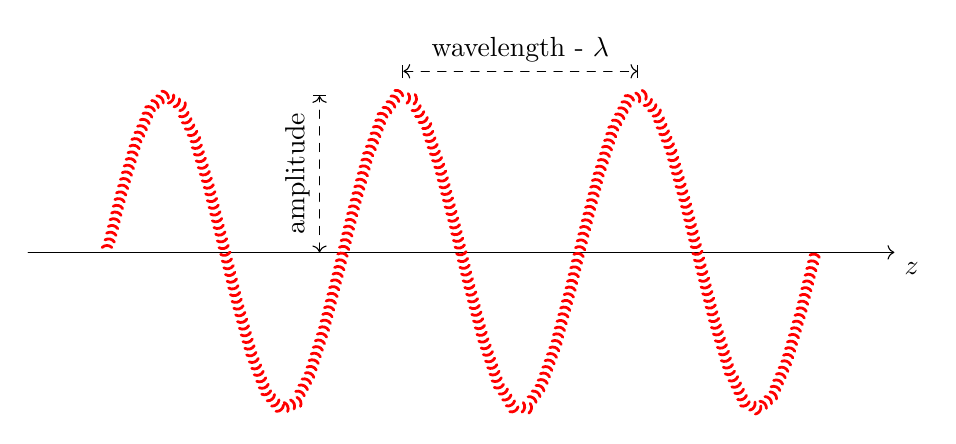
\begin{tikzpicture}[line join=round, line cap=round]

  % draw coordinate
  \draw[->] (-1,0) -- (10,0) node[pos=1.02,below] {$z$};
 % \draw[->] (0, -1) -- (0,2);
  % Rope properties
  \def\length{9}  % Length of the rope
  \def\thickness{1}  % Thickness of the rope
  \def\waveAmplitude{2}  % Amplitude of the wave
  \def\waveLength{3}  % Wavelength
  \def\segments{50}  % Number of segments
  
  % Draw the rope
  \draw[decorate, decoration={waves, segment length=2.5}, line width=\thickness, red]
    (0,0) -- plot[domain=0:\length, samples=\segments]
    (\x, {\waveAmplitude*sin(\x*(360/\waveLength))}) -- (\length,0);

    % label
    %\draw[red, fill] (3.75,2) circle(0.05cm);
    %\draw[red, fill] (6.75,2) circle(0.05cm);
    %\draw[dashed] (2,2) -- (3.75,2);
    \draw[<->|, dashed] (2.7,0) -- (2.7,2) node[pos=0.5, rotate = 90, above] {amplitude};
    \draw[|<->|, dashed] (3.75,2.3) -- (6.75,2.3) node[pos=0.5, above] {wavelength - $\lambda$};

\end{tikzpicture}

    \caption{Caption}
\end{figure}

但一个振动的琴弦是不是波呢?是的,我们看不到振动传播是因为弦两端被固定,向一个方向传播的振动被固定一端反射成相反方向传播的波,相向传播的两波叠加显现成不传播的固波。这种波就复杂一些,它的波长也被限制只能取一些特定值。这个例子告诉我们,两个或多个波的叠加合成也是波,当然一个波也可以分成多个子波,而且合成的波参量特性会与子波的不同。

被原子核电荷吸引力束缚的电子波也类似驻波。1897年,英国剑桥大学开文迪许实验室的汤姆逊做的真空管实验发现了电子,他观察到的电子是一粒一粒的,并测量出每一粒相等的质量。现在我们知道,电子是波,尺寸不一定小,如果没有带正电的原子核束缚或者真空管里磁场束缚,它会稀疏的漫延或传播到整个宇宙。可是建立电子波性理论却用了汤姆逊之后的三十年时间,欧洲几个国家几十位顶级科学家的努力,从1911年提出的波尔模型,到1926年发表的薛定谔波动方程再到1928年的狄拉克方程。

电子的波性很复杂,量子物理教程通篇大部分是讲如何解电子波动方程。本书多以电磁波为例,避免涉及电子波。做为信息技术工程师,我们只需要知道波有哪些参数可以用来承载信息,而将解波动方程的事交给物理系学生。

\subsection{量子性}
量子性除了说每种波的能量或质量这个参量都是某最小单位的整数倍,别无它意。本来这个概念很简单,一句话就全概括了, 而波性很丰富复杂,大学量子物理教程大部分是教如何解波动方程,需要很多计算,美国康奈尔大学默明教授的“闭嘴吧,去算!”忠告就是这个意思。遵循这个忠告的科学家成功的将量子理论做为发明各种现代科技的理论基础,从半导体技术到激光技术。可是不遵循这个忠告的众多物理学家,将本来简单的量子性称为粒子性,又因“粒子”这个词节外生支引出各种诠释,各种不休的争论。结果是量子变成了神神秘秘的高深不可知。

其实各种迷惑和荒谬的解释都源于语言隐含歧义的误导。很多人从粒子性这个名词,就会联想到其它意思,尤其是它的尺寸很小和它不可以分裂处于多个空间位置。其实单光子和单电子双缝实验早已经证明,一个“粒子”是波,它的尺寸可以很大,它可以同时向两个方向传播并同时通过两个狭缝。牛顿说光是一粒一粒的物质,是完全错的,因为“粒”隐含着尺寸小的联想。把光想象成一滴一滴的也是错的,想象成一层一层还是错了,这些量词都隐含某些尺寸的错觉。光的量子性是说我们不能把电灯的光无限的拧弱,灯光的能量或与之成正比的强度是某单位的整数倍,弱到只有一个单位就不能再弱了,否则就完全熄灭了。

17世纪末惠更斯正确的提出光是波,问题是大家日常见到的水面波纹,看不见有最弱的,只有看不见的更弱的,人们的经验就植入了波可以无限弱这个错觉。但是19世纪末科学家做的黑体光辐射与频率关系的实验结果发现与含有那个假设的理论推导不符。那时候德国的普朗克(Max Planck, 1858-1947)已经是享誉世界的科学家了,他1900年发表的论文没敢明确说光能量不能无限小,而是说如果先假设某频率的光能量是$hf$的整数倍, 再用波动理论推导的结果就与实验相符了。这里$f$是光振动频率,$h$是当时普朗克假设的一个正比系数,时至今日h就是已被精确测定大名鼎鼎的普朗克常数。现在德国以普朗克命名的实验室更在物理和化学生物人文等众多学科中成为世界顶级科研机构

1900年,20岁的爱因斯坦(Albert Einstein, 1879-1955)刚读完大学。为逃避征兵他已经放弃德意志符腾堡王国国籍移居瑞士4年了,还要等一年他才会取得瑞士国籍。后面几年,他一边做专利局审议助理,一边专研物理写论文。1905年是他论文爆发年,连发5篇论文外加一篇苏黎世大学博士论文,其中4篇是奠基性的,包括奠定和超越狭义相对论的“狭义相对论”和 “质量与能量等价”两篇。给量子理论奠定基础的是他的“光电效应”论文。他指出普朗克假设的实质是光能量有最弱单位,称为光量子,只有当光频率大于某阈值频率,一个光量子才有足够能量来使得一个电子摆脱原子核束缚,产生光电效应的电流。爱因斯坦的论述解释了为什么光电效应实验结果显示阈值只与光频率有关,而与光强度无关。现在物理学家多用光子,而舍弃光量子这个名称。我们认为光子总给人尺寸小的印象,更希望回到爱因斯坦原始的光量子一词。

\section{量子比特}
\subsection{用波参量承载信息}
在\ref{string}里,波长这个参量描述传播一周期的距离,振幅描述振动的幅度。图中没有标识的,还有一个叫偏振的参数,表述的是绳子振动的方向,一般用振动方向与水平线的角度衡量。下章我们会进一步讨论,有两个参量描述波随时间的振动:频率描述每秒钟振动次数,与波长成反比;相位描述振动在时间上的延迟。

不同通信技术会选不同电磁波参量承载信息,最常用的是振幅,频率,相位和偏振。本书举例的量子比特用相位和偏振承载信息,实际制造的,根据材料不同,会用频率还有一个叫模式的参量替代偏振。表-\ref{t-modulations}列出一些通信技术和光量子比特信息承载参量和取值。对于熟悉通信技术的学生,通信与量子技术的一致性和不同一目了然。对于没有学过通信理论的,表中的很多名词很陌生。我们不妨在学习下面两章后,在回过来看这个表。
\begin{table}[]\label{t-modulations}
\begin{tabular}{|l|l|l|l|l|}
\hline
调制技术 & 频率 & 振幅 & 相位 & 偏振   \\ \hline
调幅广播(AM) &  & 近似于[0, $\infty$) &  & \\ \hline
调频广播(FM) & (0, $\infty$) &  &  &  \\ \hline
256QAM Wi-Fi & OFDM多路复用 & \multicolumn{2}{l|}{选256 对值} & \\ \hline
OTN4, 100GbE光纤通信 & WDM多路复用 &  & $\pi/4, 3\pi/4, 5\pi/4, 7\pi/4$ & $\pi/4, 3\pi/4$ \\ \hline
光量子比特 &  & 多路复用 & [0, $2\pi$) & [0, $\pi$) \\ \hline
\end{tabular}
\end{table}


\subsection{用波参量变换实现运算}
针对不同的应用,选用的调制方法包括数字与载波参量的对应关系会不同。最常用的光量子比特的对应关系是用偏振0,45,90,和135度角分别对应00,11,01和10四个二进制数。如果将一个光量子比特的偏振角转90度,那么它对应的数字就从11变成10,实现11-01=10的运算。从这个例子,我们看到一个量子比特可以承载起码2位数数字并进行计算,比普通计算机的单比特要多。当然这个例子貌似粗陋不堪,我们恐怕要等到后面几章学习具体的算法时,才能体会多个简单波参量变换可以组合实现复杂运算。

近一百年前,英国科学家图灵(Alan Turing, 1912–1954) 发明了抽象的图灵机用于(信息处理)算法研究。只有通过图灵机验证的,才是数字符号层面上能实现的算法,否则是不能编程实现的。我们每天用的计算机可以实现任何图灵算法,是图灵完备的,量子计算机也是。量子比特的波参量变换都可以表现为数字符号层面上的U矩阵变换,科学家已经证明U矩阵变换的组合可以实现任何图灵运算。这里算法也包含通信协议,只不过后者的步骤需要发送方和接收方分别完成,而一般意义上的算法不限定由谁完成。

\subsection{量子优势}\label{sec:whyquantum}
信息技术现在差不多都从模拟技术转用数字技术,虽然现在还有人在听调幅调频广播,不久前我们还在用有水银柱的血压仪。我们的印象是模拟技术是牙齿差不多掉光的技术,我们该全盘接受先进的数字技术。事实上,模拟技术有信息承载量大的优点,只是碍于噪声我们不得不用数字技术。如果没有噪声,模拟技术能承载更多信息,或者说数字技术用牺牲信息承载量的代价换取准确无错的优点。

有什么办法兼有模拟技术承载信息量的优势,又能避开噪声呢?物理学告诉我们噪声是随机能量,尤其是热能。所以信息元件不该用与能量相关的物理参数比如波的振幅承载信息。物理学告诉我们电磁波有很多参数如相位和偏振角度,都与能量无关。用一个光量子的相位和偏振承载信息,就是量子比特的构造。

相位是波震动时间的延迟或者说是传播距离的延长,改变波传播路程就可以改变相位;改变光程长是不损耗能量的,就像一个汽车因为惯性多滑行几百米改变了里程表显示,却不需能量注入。偏振是电场的方向,弯曲甚至扭曲一个光纤光缆,可以改变光传播方向和偏振方向,也不增减光的能量。几百年里,物理学家发明了所有能改变光波相位和偏振参数的元件,比如相位板(phase plate)和波片(wave plate)。量子比特运算的过程是变换它的相位和偏振参量的过程,不需能量交换就避开了最大的噪声来源。

\subsection{量子比特读取瓶颈和测量}
量子比特读取瓶颈归根是量子物理中的测量问题,其深刻机制是所有测量都存在测量对象与测量设备之间的能量交换,测量设备根据是否从对象获取能量或成功给与能量认定测量结果,而一个量子比特只有一份能量可供测量。冯·诺伊曼对测量问题有极深入的研究,他将测量看成一种投影是准确的。

很多物理量不是一次测量就能够有结果的。我们的GPS要确定位置,需要测量起码三个卫星与我们的距离,也就是说确定三维空间里一点需要三个测量。波偏振和相位各自是二维平面上一点,都需要起码两个测量。比如测量偏振角度就需要在0⁰和90⁰两个垂直方向上放两个探测器,测量振动电场在两个方向的分量比。测量过程需要用波的能量将被束缚的电子变成可流动的电子,进而产生电流信号,是能量转换过程。因为一个量子比特只有一个单位能量,两个分量测量接收器中只有一个能测量到,一份能量不能被两个接收器收下,不可能得到分量比。所以,在测量之前,波的偏振是确定的,它承载的信息也是确定的,但当波的偏振等于0⁰或90⁰,才能够准确测量,其它偏振角度的测量都不会有准确结果,相位的测量同样失去意义。因为这个读取限制,计算结果的量子比特偏振必须是0⁰或90⁰,只有与它们对应的数字00和01能够读取,而11和10不能读取。

我们可以用薛定谔猫来比喻这个量子现象:这个猫有几条命是确定的量,是我们要得到的信息;可是测量过程是一次性的而且像盲人摸象那样片面的,我们只能得到0或9条命的结果,所以除了在这个猫有0或9条命时,我们的测量都是不准确的。

\section{量子技术与应用}
量子计算是公认会带来巨大经济效益的技术。量子通信的经济效益目前还不很显著,原因包括1)目前的通信加密技术已满足几乎所有要求,2)量子通信加密的大部分技术指标如密码传递距离还很差,3)造价很高。量子信息学还有一个潜在的应用目前大家还没有意识到,那就是它会给下一代芯片设计和制造提供理论基础。目前的芯片是用半导体三极管元件里面的众多电子积累的物理量,如电压和电流,承载信息。进一步做小于几纳米尺寸的芯片元件,电子数很少的话,就必须用少数电子的波参量承载信息,那就需要量子信息理论了。

\subsection{量子比特制备}
制备量子比特的关键是将每个量子波与其它的分开从而可以分别读取测量它的物理量,一般是将它们在空间上分开。目前的量子比特都是用光波或电子波。电子有电荷,很容易受携正电荷的原子核束缚稳定的集中在某空间区域,所以最适用于量子计算,而不会用于量子通信。用光量子制备的量子比特是量子通信唯一选择;而用于量子计算,它有噪声干扰小的优点,但将光量子局限在某空间区域是个不小的技术挑战。用于量子计算的量子比特主要选择是由原子核束缚电子的囚禁离子和中性原子技术,超导体束缚电子成准粒子技术,和由2-维光波导束缚的光量子。

\subsection{量子计算编程}
用于计算,量子电路会做成像GPU一样的QPU协处理器,加速运算。软件编程表面跟用GPU差别不大,但是实际上需要深入的量子算法知识。一个AI编程只需要高层的算法知识,运算细节隐藏在Python程序调用的PyTorch软件包里:
\begin{lstlisting}
# 调用软件波
import torch
import math
# 如果配置有GPU,调用GPU加速运算,否则用CPU
device = "cuda" if torch.cuda.is_available() else "cpu"
torch.set_default_device(device)
# 建立一个3x4张量
x = torch.empty
\end{lstlisting}

调用IBM量子计算机的QISKIT软件包的Python程序则需要写出算法的每一步,比如一个多伊奇Deutsch算法程序会是这样的
\begin{lstlisting}
# 调用软件波
from qiskit import QuantumCircuit
# 用一个量子比特和零个普通比特建立一个运算电路
qc = QuantumCircuit(1, 0)
# 用Hadamard量子门将量子比特偏振转45⁰,表示的编码是10—等价于同时输入1和0两个数给下一步骤
qc.h(0)
# 对1和0两个输入数同时做运算
qc.x(0)
# 用Hadamard量子门将量子比特偏振再转45⁰
qc.h(0)
# 测量量子比特的值,给出 0或1 结果
qc.measure([0, 1])
# 画出电路图
print(qc.draw())
\end{lstlisting}

所以理解量子算法的步骤是程序员编程必须的知识。

\chapter{用偏振波承载信息}\label{c-modulation}
一百多年前马可尼(Guglielmo Marconi, 1874-1937)发明的电报技术就是用无线电磁波的振幅承载信息,我们现在每天用的通信全是用电磁波参量承载信息,通信的调制技术和理论对用波承载信息有最系统而实用的指导。调制技术解决这些问题:
%
\begin{table}[]\label{t-modulation-steps}
    \caption{调制技术解决的问题}
\begin{tabular}{|l|l|l|}
\hline
问题 & 无线通信方法和思路 & 光量子比特方法和思路   \\ \hline
选择哪些波参量能达到承载信息量的要求 &  振幅+相位 &  偏振+相位 \\ \hline
选择哪些波参量值能避开其它限制 & 避开噪声限制 &  避开读取限制  \\ \hline
选择波参量值怎样与信息符号对应 & 易纠错 & 依算法定 \\
\hline
\end{tabular}
\end{table}

对于通信专业的学生,本章复习调制的基本方法,先分开讲解简单相位和偏振调制,然后归结到合用两个参量的椭圆偏振调制-用于光量子比特。其它种类量子比特与光量子承载信息的原理是一样的,只不过会用与偏振等价的其它波参量与相位结合承载信息。对于非通信专业学生,本章引入很多通信理论的方法和术语,给后面章节量子比特信息承载奠定基础。

\section{波函数,参量和调制}
图-\ref{string}显示的是一个最简单沿$z$方向传播的波--振动高度依正弦函数随距离$x$变化,其中$A$是振幅\index{振幅},$\lambda$是波长\index{波长}.图中有显示,但没有标识的是波的偏振 -- 振动的方向,图中演示的是$y$方向,但实际上可以是垂直于传播方向的任何方向。可是振动高度也随时间$t$变化,写成波函数就是,
\begin{equation}\label{e-hWave}
    h(z,t) = A cos[2\pi (\frac z \lambda - \frac t T) +\phi]
\end{equation}

图-\ref{Wave}显示的是振动随时间的变化,$T$是周期\index{周期},而$\phi$是相位\index{相位}。
\begin{figure}\label{Wave}
\begin{tikzpicture}[scale=1.2]
    \draw[->] (-3.8,0) -- (3.9, 0)  node[pos=1.02,below] {$t$};
    \draw[->] (0,-3.5) -- (0,3.5)   node[pos=1.02,right] {$h$};
    \draw[dotted, red] (-3.5,0) sin (-2.5,3) cos (-1.5,0) sin (-0.5,-3) cos (0.5,0) sin (1.5,3) cos (2.5,0) sin (3.5,-3);
    \draw[red, fill] (-2.5,3) circle(0.05cm);
    \draw[red, fill] (1.5,3) circle(0.05cm);
    \draw[dashed] (-2.5,0) -- (-2.5,3) node[pos=0.5, rotate = 90, above] {振幅 - $A$};
    \draw[dashed] (-2.5,3) -- (1.5,3) node[pos=0.3, above] {周期 - $T$};
    %\draw[gray, fill] (1.5,0) circle(0.05cm);
    \draw[dashed] (-2.5,0.6) -- (0, 0.6) ;
    \draw[dashed] (-1.2, 0.5) -- (-2, -2) node[below] {相位 - $\phi / T$};
\end{tikzpicture}
    \caption{正弦振动}
\end{figure}

用这些参量承载信息,就是通信的调制技术。但是其中波长与周期成正比,而与频率成反比,一般只提频率调制。相位是一个波在一个周期里的进程,相位调制最基本,但所有现代调制技术都用相位复合其它参数,包括量子比特。

\subsection{星座图}
现代无线通信,包括Wi-Fi和4G以后的手机通信,都用振幅加相位正交幅度调制(Quadrature Amplitude Modulation - QAM)。通信教科书里会用选取代表信息的振幅和相位值做为极坐标的极经和极角,画出所谓的星座图。每个选取的坐标点就是一个星座,对应一个信息符号层面的数字符号。取16个星座的叫16QAM,图-\ref{16qam}是它的星座图。16个星座间要有足够间距才能避开噪声,每个星座的大小标志着它抗噪声的能力。星座越多,一个传递时间段能传输的信息越多。如果我们注意看手机的技术指标,也许看到它支持64QAM, 256QAM,甚至512QAM调制,那就是说一个手机信号波可以有64, 256, 和512个星座承载数字信息。星座越多,手机能达到的网速就越高。新一代Wi-Fi 7可以支持4096QAM。

\begin{figure}
    \label{16qam}
%\label{16QAM}
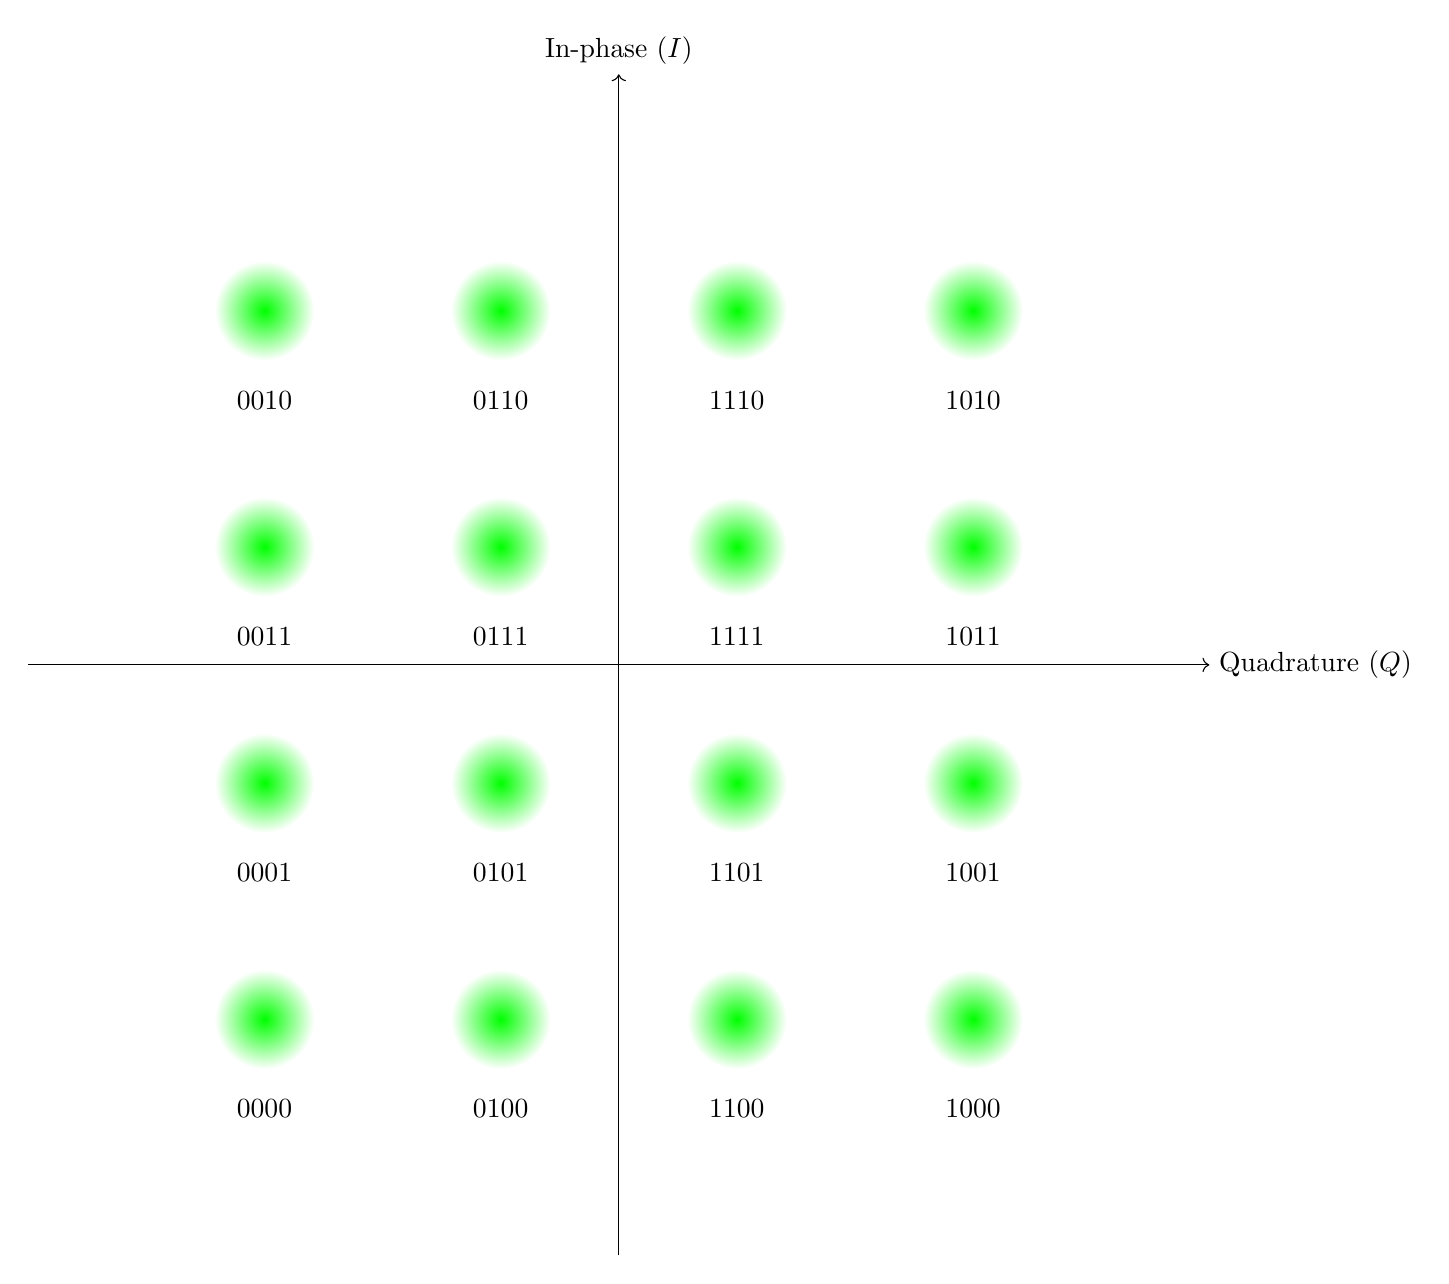
\begin{tikzpicture}[scale=3]
% Axis
\draw[->] (-2.5,0) -- (2.5,0) node[right] {Quadrature ($Q$)};
\draw[->] (0,-2.5) -- (0,2.5) node[above] {In-phase ($I$)};
% Constellation points and labels
\foreach \x/\ix in {-1.5/00, -0.5/01, 0.5/11, 1.5/10} {
    \foreach \y/\iy in {-1.5/00, -0.5/01, 0.5/11, 1.5/10} {
        \shade[shading=radial, inner color=green, outer color=white]  (\x, \y) circle (6pt); % Larger circle with fading edge
        \node[anchor=north] at (\x, \y - 0.3) {\ix\iy}; % Shift labels slightly below
    }
}
\end{tikzpicture}
    \caption{16QAM星座图。通信工程师称相位为零的波为同相波(in-phase wave),相位为$\pi/2$的叫正交波(quadrature wave)。}
\end{figure}

\section{相位调制}
\subsection{模拟型相位调制和数学表述}\label{sec-PM-notions}
相位是$[0,2\pi)$之间的实数,模拟型相位调制用所有值承载信息。图-\ref{PM}它的星座图中,半径为$A$的圆上所有点都是可以承载信息的星座。
\begin{figure}\label{PM}
\begin{tikzpicture}
    \draw[->] (-3.5,0) -- (3.5, 0);
    \draw[->] (0,-3.5) -- (0,3.5);
    \draw[dotted, red] (0,0) circle(3cm);
    \draw[red, fill] (30:3) circle(0.05cm);
    \draw[dashed] (1,0) arc (0:30:1) node[right, pos=0.6]{$\varphi$ - phase};
    \draw[dashed] (30:0.1) -- (30:2.9) node[pos=0.5, rotate = 30, above] {amplitude};
\end{tikzpicture}
    \caption{相位调制星座图,圆上所有星座点都可以承载信息。}
\end{figure}
圆上每个星座点极坐标是$(A, \phi)$,写成直角坐标是$(A cos\phi, A sin\phi)$,它也可以写成复数$A e^{i\phi}$。极坐标画在星座图上直观易懂,复数表述则更适合数学演算,是后面复杂问题的主要表述方式。

\subsection{QPSK调制}
四相相移键控(quadrature phase-shift keying - QPSK)是几个过时的Wi-Fi标准用的数字调制技术,它可以用来代表两位二进制数字,0, 1, 10, 11,它也可以看成是4QAM调制。最简单的QPSK是如图-\ref{QPSK}所示取$\phi = 0, \pi/2, \pi, 3\pi/2$ 为星座。更为实用的是如图-\ref{sQPSK}所示的所谓对称四相相移键控(Symmetric QPSK),它以$\phi = \pi/4, 3\pi/2, 5\pi/4, 7\pi/4$ 为星座。

\begin{figure}[h]\label{QPSK}
\begin{tikzpicture}
    \draw[->] (-3.5,0) -- (3.5, 0);
    \draw[->] (0,-3.5) -- (0,3.5);
    \draw[dotted, red] (0,0) circle(3cm);
    \draw[red, fill] (3,0) circle(0.05cm) node[below right] {0};
    \draw[red, fill] (0,3) circle(0.05cm) node[above right] {1};
    \draw[red, fill] (-3,0) circle(0.05cm) node[above left] {10};
    \draw[red, fill] (0,-3) circle(0.05cm) node[below left] {11};
\end{tikzpicture}
%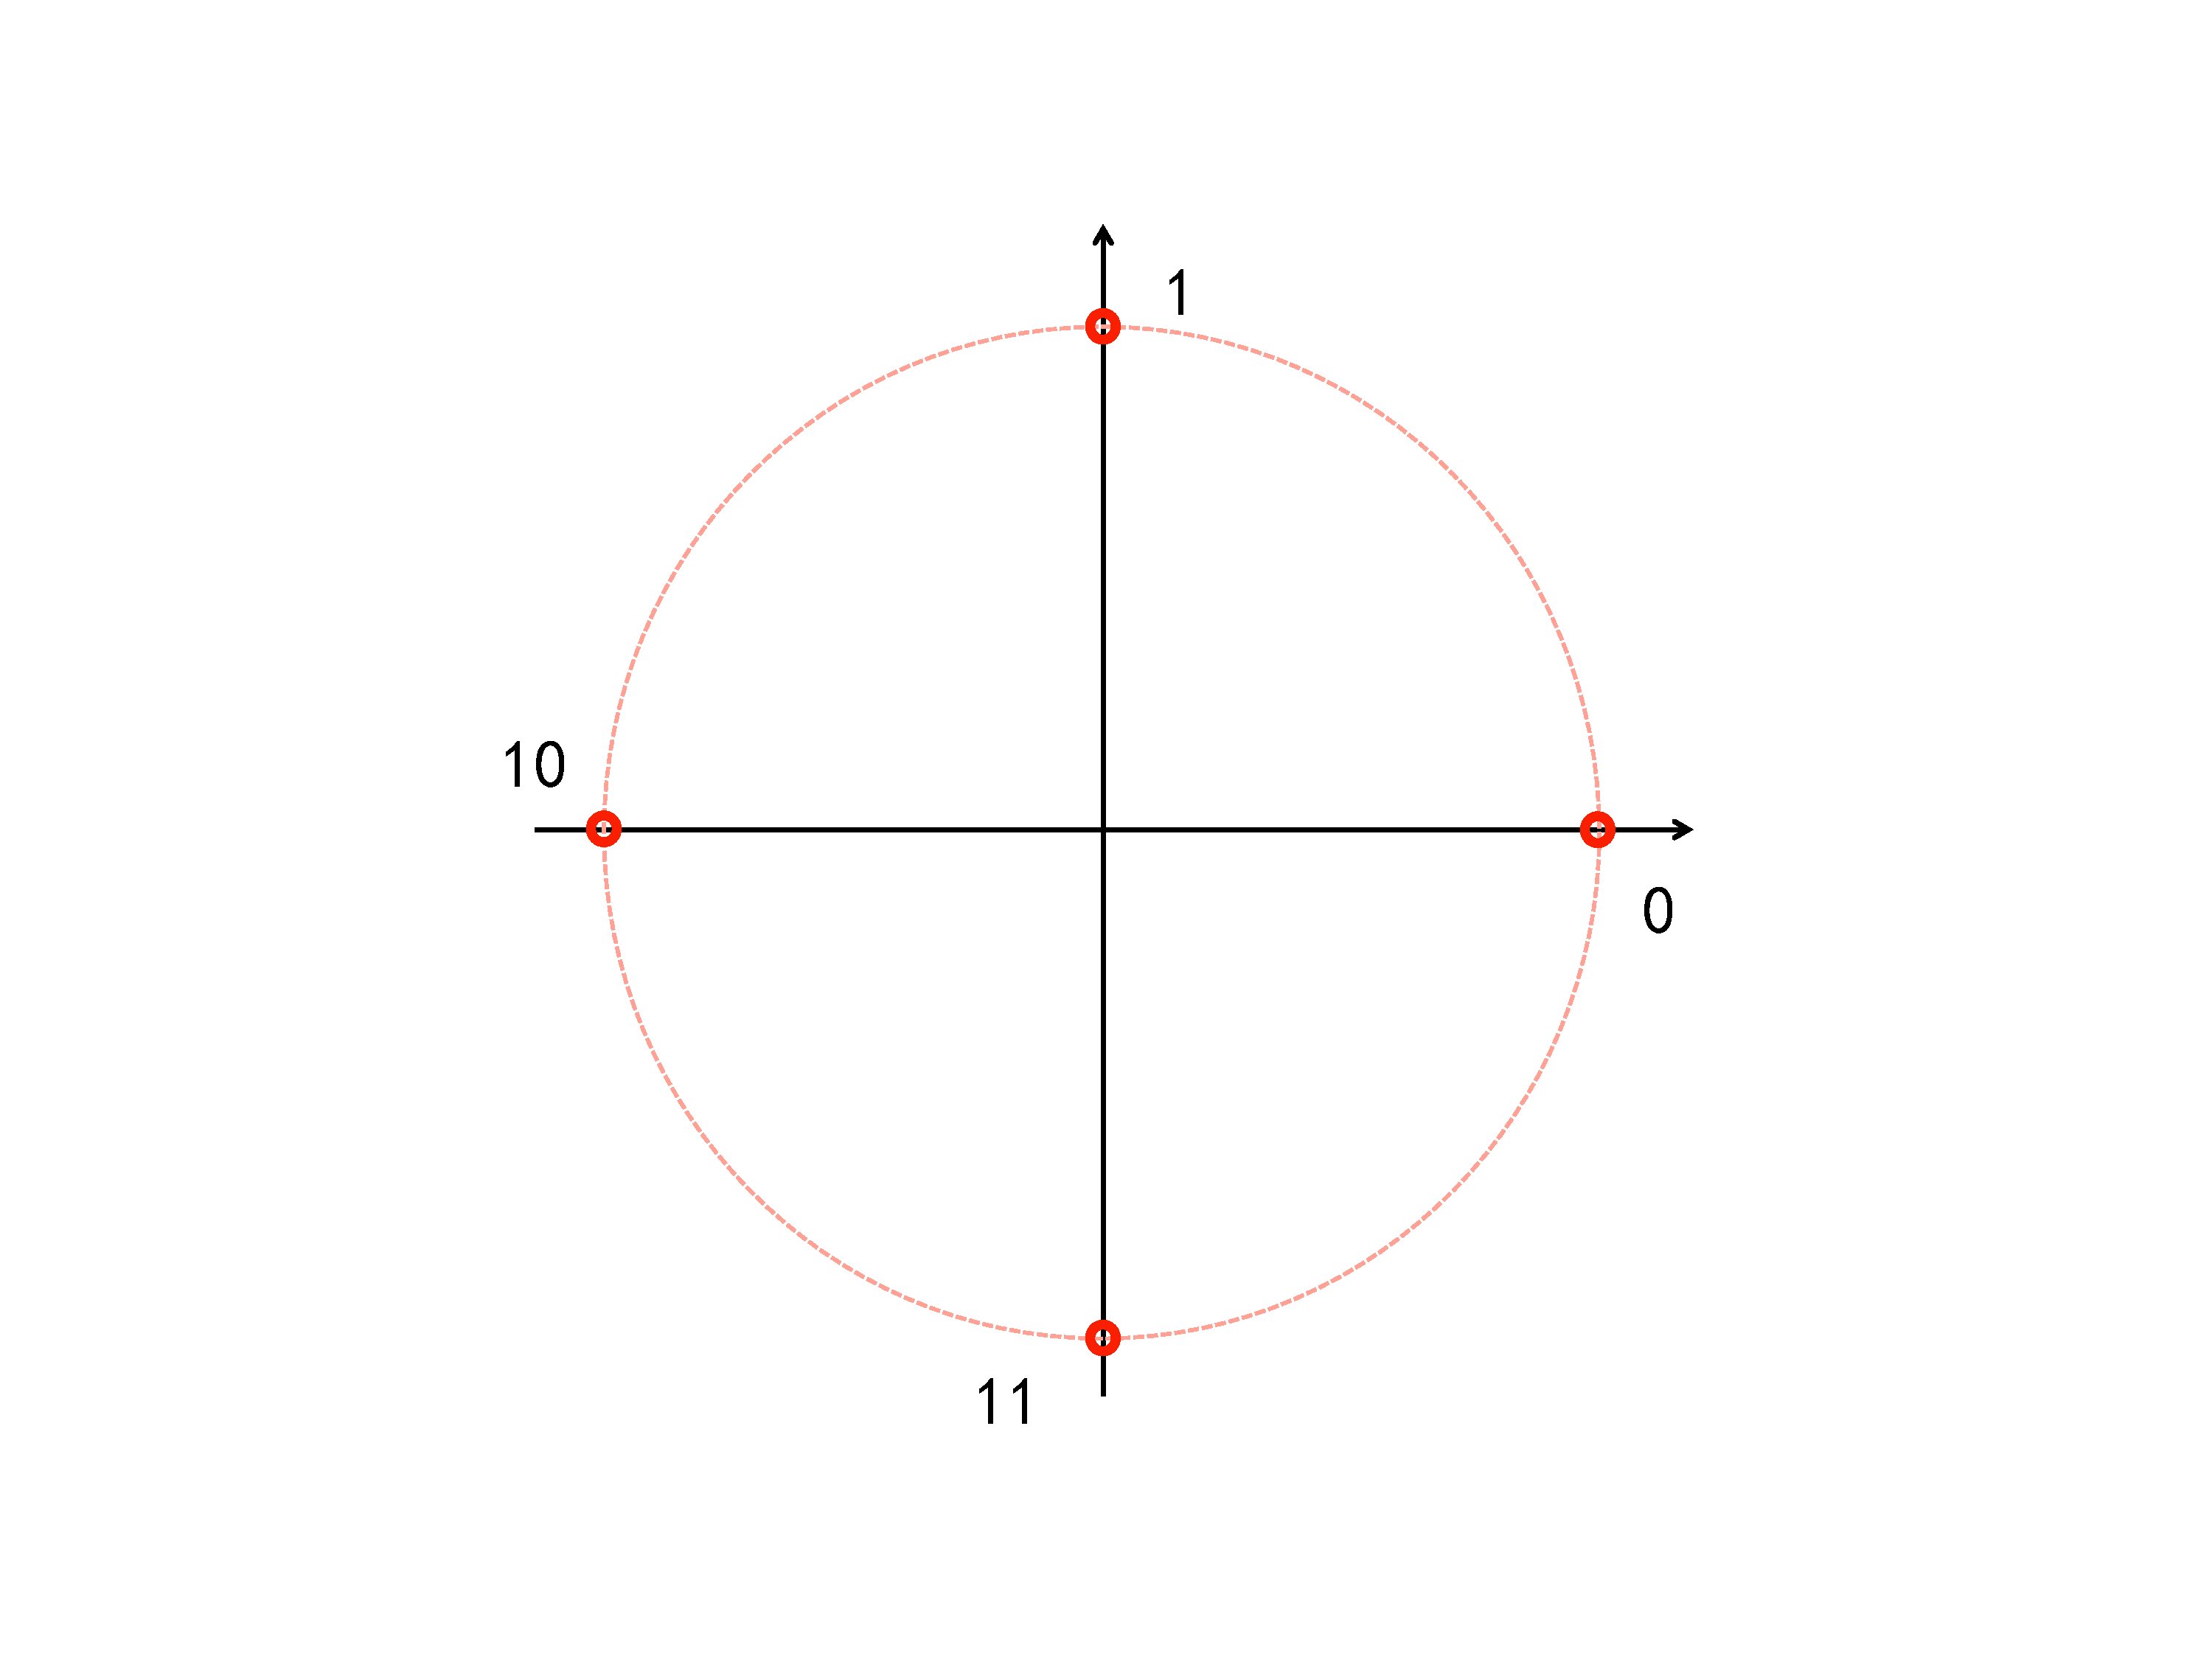
\includegraphics[width=6cm]{pic/4qpsk.pdf}
\caption{QPSK constellation diagram}
\end{figure}

\begin{figure}[h]\label{sQPSK}
\begin{tikzpicture}
    \draw[->] (-3.5,0) -- (3.5, 0);
    \draw[->] (0,-3.5) -- (0,3.5);
    \draw[dashed] (2.5,2.5) -- (0, 0);
    \draw[dotted, red] (0,0) circle(3cm);
    \draw[red, fill] (2.12,2.12) circle(0.05cm) node[right] {11};
    \draw[red, fill] (-2.12,2.12) circle(0.05cm) node[above] {01};
    \draw[red, fill] (2.12,-2.12) circle(0.05cm) node[below] {10};
    \draw[red, fill] (-2.12,-2.12) circle(0.05cm) node[left] {00};
    \draw[dashed] (1,0) arc (0:45:1) node[right, pos=0.6]{$\varphi=45\circ$};
\end{tikzpicture}
\caption{Symmetric QPSK constellation diagram}
\end{figure}

\subsection{对称QPSK调制器和解调器}\label{Sec-demodulator}
调制器是按输入的数字符号,把波的参量变成对应的星座值的元件,解调器做相反的功能。量子技术的调制器和计算处理器与通信用调制器都是基于同样原理和元件,我们下章会更详细讲解。但是解调器则与通信用解调器有重大不同,这章我们会多花笔墨介绍通信用解调器。

从\ref{sec-PM-notions}一节,我们知道相位是个向量,可以表述成两个垂直分向量的和。事实上,任何相位的波都可以由两个相位相互成90度的波叠加合成。图-\ref{modulator}所示对称QPSK调制器就是用这个原理。按通信工程师们的习惯,称零相位的波为同相(in-phase wave)或I波,90度相位的为正交波(quadrature wave)或Q波。每个方块是一个标有功能的元件,这些元件如波源,分波器,移相器都是光量子电路用到的。
单条线代表波传播,双条线代表电子数字输送。

我们不妨设想这是一个Wi-Fi路由器里的调制器,电子数字从双条线里输入,带有信息的无线电信号波通过天线发出。每个时间段发送两个比特:偶数比特决定I波的相位为0还是180度,奇数比特决定I波的相位为0还是180度。叠加合成波的相位就可能是$\pi/4, 3\pi/2, 5\pi/4, 7\pi/4$。

\begin{figure}[ht]\label{modulator}%modulator1
\begin{tikzpicture}
    \path
    (-2,-1) node[circle, draw=black] (lo) {$\sim$}
    (0,-1) node[circle, draw=black] (splitter) {$\prec$}
    (0,1) node[Gate] (p90) {$90^\circ$}
    (0,3) node[Gate] (ta) {$180^\circ$}
    (0,-3) node[Gate] (ba) {$180^\circ$}
    (3,0) node[circle, draw=black] (coupler) {$\succ$}
     (4,0) node[text width=60, align=center, anchor=west] (output) {信号波输出signal wave output};
    \path (-2,3) node[text width=50, align=left, anchor=east] (even) {数据输入data input - even bits}
    (-2,-3) node [text width=50, align=left, anchor=east] (odd) {数据输入data input - odd bits};

    \draw (lo.north) node[text width=80, align=center, anchor=east] {载波源carrier wave generator};
    \draw (splitter.south east) node[text width=40, align=center, anchor=west] {50:50 分波器splitter};
    \draw (p90.north west) node[text width=40, align=center, anchor=east] {相位延迟phase shifter};
    \draw (ta.north) node[anchor=south] {controlled phase shifter};
    \draw (ba.south) node[anchor=north] {controlled phase shifter};
    \draw (coupler.north west) node[text width=40, align=center, anchor=east] {合波器coupler};
    \draw (coupler) -- (output);
    \draw (ba) -- (splitter) -- (p90) -- (ta) -| (coupler) |- (ba);
    \draw (lo) -- (splitter);
    \draw[double] (even) -- (ta);
    \draw[double] (odd) -- (ba);
\end{tikzpicture}
\caption{对称QPSK调制器电路图}
\end{figure}

图-\ref{Demodulator}所示解调器电路基本上是逆着调制器,它的本地波源分出相位相差90度的两个分波,后者再分别与天线接收的信号波分出的两个分波叠加合成。叠加合成波产生相干效果,正相干的合成波在后面的电子接收器中产生电流,数据输出就是"1"。如果合成波是负相干,也就是合成的分波相位差180度,电子接收器就没有电流信号,数据输出就是"0"。

我们看到相位好像是一个$[0, 2\pi)$之间的实数值,但是它是个二维向量,测量时必须将它投影到两个垂直方向上分别测量。这个特性是量子比特受限于读取瓶颈的根源。

\begin{figure}[h]\label{Demodulator}
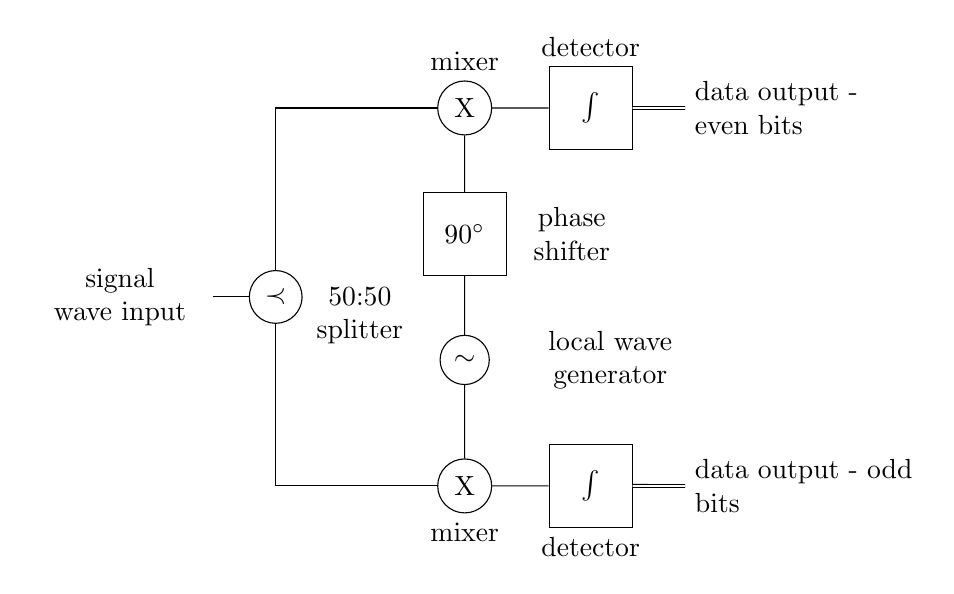
\begin{tikzpicture}[scale=0.8]
    \path
    (0,-1) node[circle, draw=black] (lo) {$\sim$}
    (0,1) node[Gate] (p90) {$90^\circ$}
    (0,3) node[circle, draw=black] (ta) {X}
    (0,-3) node[circle, draw=black] (ba) {X}
    (2,3) node[Gate] (tm) {$\int$}
    (2,-3) node[Gate] (bm) {$\int$}
    (-3,0) node[circle, draw=black] (split) {$\prec$}
     (-4,0) node[text width=60, align=center, anchor=east] (input) {signal wave input};
    \path (3.5,3) node[text width=80, align=left, anchor=west] (even) {data output - even bits}
    (3.5,-3) node [text width=80, align=left, anchor=west] (odd) {data output - odd bits};

    \draw (lo.east) node[text width=80, align=center, anchor=west] {local wave generator};
    \draw (p90.east) node[text width=40, align=center, anchor=west] {phase shifter};
    \draw (tm.north) node[anchor=south] {detector};
    \draw (bm.south) node[anchor=north] {detector};
    \draw (ta.north) node[anchor=south] {mixer};
    \draw (ba.south) node[anchor=north] {mixer};
    \draw (bm) -- (ba) -- (lo) -- (p90) -- (ta) -- (tm);
    \draw[double] (even) -- (tm);
    \draw[double] (odd) -- (bm);

    \draw (ba) -| (split)  |- (ta);
    \draw (split.south east) node[text width=40, align=center, anchor=west] {50:50 splitter};
    \draw (split) -- (input);    
\end{tikzpicture}
    \caption{Symmetric QPSK demodulator.}
\end{figure}

\section{偏振调制}
对于电磁波,偏振是振动的电场的方向,总是与波传播方向垂直的。如果用$z$代表传播方向,那么偏振总是在$x-y$平面上的。最简单的波是所谓的线性偏振波--它的电场总在一个方向上震荡,这个方向与$x$轴的角度不妨标为$\theta$。那么这个角度物理量就可以用来承载信息。

\subsection{线性偏振调制}
如同相位调制,模拟型线性偏振调制可以用如图-\ref{PolarM}的星象图直观描述,圆上每个星座点极坐标是$(A, \theta)$。与相位不同,它的取值范围是$[0, \pi)$,大于180度的偏振$\theta$与$\theta-\pi$是一样的波,也就是重复了$[0, \pi)$的那些星座。

如同相位,线性偏振是个向量,写成直角坐标是$(A cos\theta, A sin\theta)$。事实上,任何线性偏振波也都可以由两个相互成90度的线性偏振分波叠加合成,$x$方向分波振幅为$(A cos\theta$,$y$方向分波振幅为$A sin\theta)$。

如同相位,线性偏振的调制和解调器电路与图-\ref{modulator}和图-\ref{Demodulator},其中的分光器会是偏振分光器,相位延迟会是偏振器。调制是将两个垂直偏振分波合成,解调是将接收的偏振波分成两个垂直方向分波,分别与解调器自己的波源相干测量分波的振幅。

\begin{figure}[h]\label{PolarM}
\begin{tikzpicture}
    \draw[->] (-3.5,0) -- (3.5, 0);
    \draw[->] (0,-3.5) -- (0,3.5);
%    \draw[dotted, red] (0,0) circle(3cm);
    \draw[dotted, red] (3,0) arc(0:180:3);
    \draw[red, fill] (30:3) circle(0.05cm);
    \draw[dashed] (1,0) arc (0:30:1) node[right, pos=0.6]{$\theta$};
    \draw[dashed] (30:0.1) -- (30:2.9) node[pos=0.5, rotate = 30, above] {振幅amplitude};
\end{tikzpicture}
\caption{模拟型线性偏振星象图}
\end{figure}

\subsection{椭圆偏振波}\label{s-elliptic}
我们知道一个线性偏振波可是分成两个垂直的线性偏振分波,那么反过来两个垂直的线性偏振分波的叠加合成还是一个线性偏振波吗?答案要看这两个分波的相位差。如果$x$和$y$方向分波的相位分别是$\phi_x$和$\phi_y$,那么它们的叠加合成波的数学表述是复数向量$(A e^{i\phi_x} cos\theta, A e^{i\phi_y} sin\theta)$。物理层面上,这是个椭圆偏振波。

椭圆偏振波的电场也是$x-y$平面上的向量,这个向量随时间变化在$x-y$平面上画出一个椭圆,而它随传播方向的变化则如图-\ref{CircularP}画出一个螺旋。当相位差$\phi=\phi_y-\phi_x$为零或180度时,这个波实际上是个线性偏振波,如果相位差为90或-90度,这个波是个圆偏振波。量子比特用$(\theta, \phi)$参量对承载信息,它的星座图是个球面。

\begin{figure}[h]\label{CircularP}
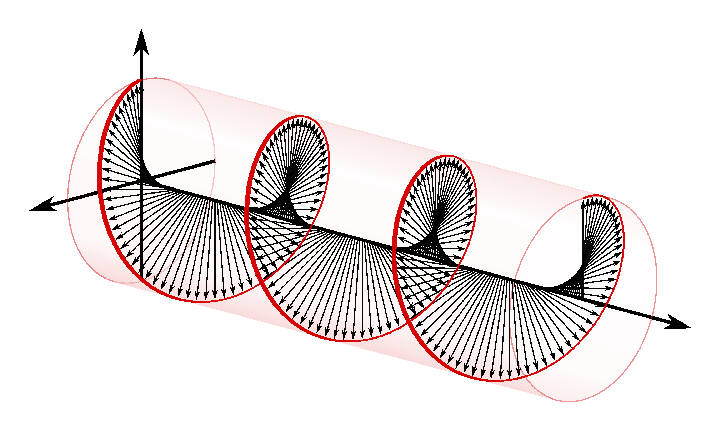
\includegraphics[width=10cm]{pic/CircularPolarization.eps}
\caption{椭圆偏振波的电场向量随着传播成螺旋变化}
\end{figure}

\subsection{DP-QPSK调制}
现代光纤通信100GbE和ONT4标准都是用称为双偏振四相相移键控(dual-polarization quadrature phase shift keying - DP-QPSK)的数字型调制,它结合偏振$\theta$加上相位$\phi$($=\phi_x=\phi_y$)承载信息。因为相位差$\phi_y-\phi_x$为零,它实际上是一个偏振调制加上一个对称QPSK相位调制。用$(A, \theta, \phi)$做为球坐标画出的星座图是个球面,上面的8个星座就是DP-QPSK取值点,如图-\ref{DP-QPSK}。

%\node [constellation_cir] at (0,0) {};
\begin{figure}[h]\label{DP-QPSK}
\tdplotsetmaincoords{75}{110}
\pgfmathsetmacro{\h}{3.53}
\pgfmathsetmacro{\hn}{-3.53}
\pgfmathsetmacro{\r}{5}
\pgfmathsetmacro{\rn}{-5}
\pgfmathsetmacro{\ang}{105}
\begin{tikzpicture}[tdplot_main_coords]
\tdplotsetcoord{P1}{\r}{45}{45}
\tdplotsetcoord{P2}{\r}{-45}{45}
\tdplotsetcoord{P3}{\r}{45}{-45}
\tdplotsetcoord{P4}{\r}{-45}{-45}

\tdplotsetcoord{P5}{\r}{135}{45}
\tdplotsetcoord{P6}{\r}{-135}{45}
\tdplotsetcoord{P7}{\r}{135}{-45}
\tdplotsetcoord{P8}{\r}{-135}{-45}

\shade[ball color=gray, tdplot_screen_coords, opacity=0.10] (0,0,0) circle [radius=\r];

% xy plane
\tdplotdrawarc[gray]{(0,0,0)}{5}{-75}{\ang}{};
\tdplotdrawarc[dashed, gray]{(0,0,0)}{\r}{\ang}{285}{};
% yz plane
\tdplotsetthetaplanecoords{90}
\tdplotdrawarc[tdplot_rotated_coords, gray!70]{(0,0,0)}{\r}{-38}{157}{};
\tdplotdrawarc[tdplot_rotated_coords,dashed, gray]{(0,0,0)}{\r}{150}{335}{};

% xyz axes
\draw[dashed, gray!50] (\rn,0,0) -- (0,0,0); \draw[gray!50] (0,0,0) -- (\r,0,0);
\draw[gray!55] (0,\rn,0) -- (0,\r,0);
\draw[gray!60] (0,0,\rn) -- (0,0,\r);
\draw[thick, -Stealth] (\r,0,0) -- (9,0,0) node[black, left] {$x$};
\draw[thick, -Stealth] (0,\r,0) -- (0,7,0) node[black, right] {$y$};
\draw[thick, -Stealth] (0,0,\r) -- (0,0,7) node[black, left] {$z$};

% points
\fill[red] (P1) circle (0.1); \fill[red!50] (P2) circle (0.1);
\fill[red] (P3) circle (0.1); \fill[red!50] (P4) circle (0.1);
\fill[red] (P5) circle (0.1); \fill[red!50] (P6) circle (0.1);
\fill[red] (P7) circle (0.1); \fill[red!50] (P8) circle (0.1);
\node[above] at (P1) {$(\frac \pi 4, \frac \pi 4)$};
\node[below] at (P2) {$(\frac \pi 4, \frac {5\pi} 4)$};
\node[above right] at (P4) {$(\frac \pi 4, \frac {3\pi} 4)$};
\node[below left] at (P3) {$(\frac \pi 4, \frac {7\pi} 4)$};
\node[above] at (P5) {$(\frac {3\pi} 4, \frac \pi 4)$};
\node[above] at (P6) {$(\frac {3\pi} 4, \frac {5\pi} 4)$};
\node[above right] at (P8) {$(\frac {3\pi} 4, \frac {3\pi} 4)$};
\node[below left] at (P7) {$(\frac {3\pi} 4, \frac {7\pi} 4$};

\draw[dashed, red!70] (0,0,0) -- (2.5, 2.5, 0) -- (P1) -- cycle;
\draw[dashed, red!30] (0,0,\h) circle (\h);
\draw[dashed, red!30] (0,0,\hn) circle (\h);

\tdplotsetthetaplanecoords{45}
\tdplotdrawarc[tdplot_rotated_coords, -Latex]{(0,0,0)}{2}{0}{45}{anchor=north east}{$\theta$}

\draw [thick, -Latex, canvas is xy plane at z=0] (2,0) arc [start angle=0, end angle=45, radius=2];
\node at (2,0.5,-0.3) {$\phi$};

\end{tikzpicture}
\caption{DP-QPSK星座图}
\end{figure}

\subsection{DP-QPSK调制器和解调器}
图-\ref{Modulator-DP-QPSK}显示的是个DP-QPSK调制器电路图,它是一个偏振调制器与两个QPSK调制器的结合。图-\ref{Demodulator-DP-QPSK}是个解调器,也是一个偏振解调器与两个QPSK解调器的结合。元件包括偏振器都是光量子电路用来制备量子门的元件,但下一章我们会讲到,(在QPSK)解调器里的本地波源则是量子比特读取器里没有的。

\begin{figure}\label{Modulator-DP-QPSK}
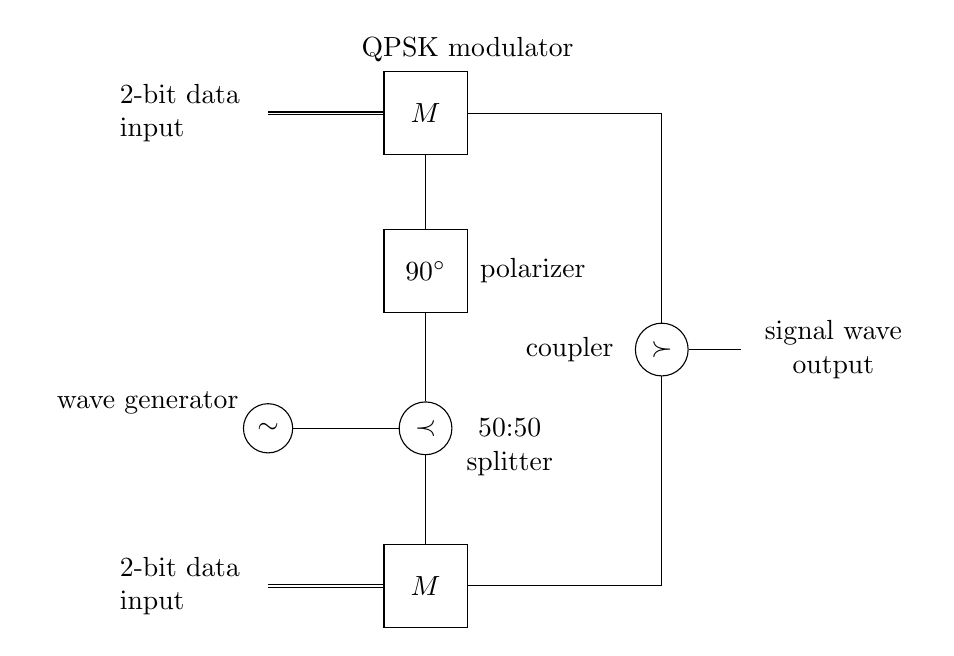
\begin{tikzpicture}
    \path
    (-2,-1) node[circle, draw=black] (lo) {$\sim$}
    (0,-1) node[circle, draw=black] (splitter) {$\prec$}
    (0,1) node[Gate] (p90) {$90^\circ$}
    (0,3) node[Gate] (ta) {$M$}
    (0,-3) node[Gate] (ba) {$M$}
    (3,0) node[circle, draw=black] (coupler) {$\succ$}
     (4,0) node[text width=60, align=center, anchor=west] (output) {signal wave output};
    \path (-2,3) node[text width=50, align=left, anchor=east] (even) {2-bit data input}
    (-2,-3) node [text width=50, align=left, anchor=east] (odd) {2-bit data input};

    \draw (lo.north) node[text width=80, align=center, anchor=east] {wave generator};
    \draw (splitter.south east) node[text width=40, align=center, anchor=west] {50:50 splitter};
    \draw (p90.east) node[text width=40, align=center, anchor=west] {polarizer};
    \draw (ta.north east) node[anchor=south] {QPSK modulator};
    \draw (coupler.west) node[text width=40, align=center, anchor=east] {coupler};
    \draw (coupler) -- (output);
    \draw (ba) -- (splitter) -- (p90) -- (ta) -| (coupler) |- (ba);
    \draw (lo) -- (splitter);
    \draw[double] (even) -- (ta);
    \draw[double] (odd) -- (ba);
\end{tikzpicture}
    \caption{DP-QPSK调制器}
\end{figure}

\begin{figure}\label{Demodulator-DP-QPSK}
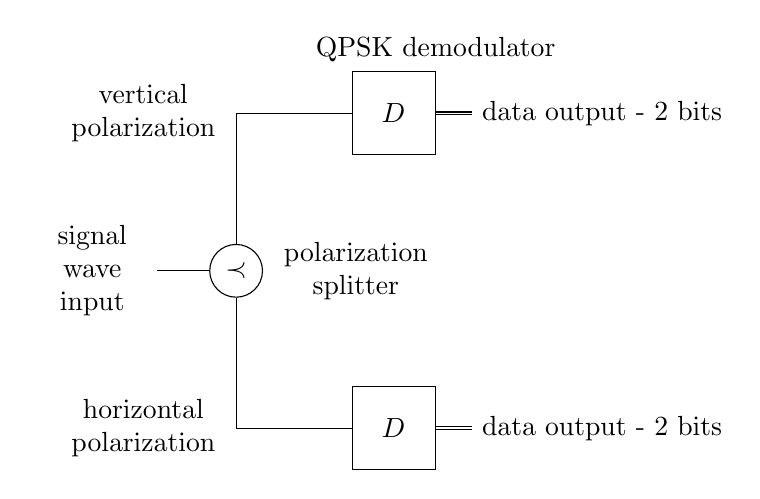
\begin{tikzpicture}[scale=1]
    \path
    (-3,0) node[text width=40, align=center, anchor=east] (input) {signal wave input}
    (-2,0) node[circle, draw=black] (split) {$\prec$}
    (0,2) node[Gate] (tsp) {$D$}
    (0,-2) node[Gate] (bsp) {$D$};
     
    \path 
    (-2,2) node [text width=60, align=center, anchor=east] (V) {vertical polarization}
    (-2,-2) node [text width=60, align=center, anchor=east] (H) {horizontal polarization}
    (1,2) node [anchor=west] (bit01) {data output - 2 bits}
    (1,-2) node [anchor=west] (bit00) {data output - 2 bits};

    \draw[double] (tsp) -- (bit01);
    \draw[double] (bsp) -- (bit00);
    
    \draw (input) -- (split) |- (tsp);
    \draw (split) |- (bsp);
    \draw (split.east) node[text width=60, align=center, anchor=west] {polarization splitter};
    \draw (tsp.north east) node[anchor=south] {QPSK demodulator};
\end{tikzpicture}
    \caption{DP-QPSK解调器}
\end{figure}

\chapter{单量子比特技术}\label{c-qinfo}
上一章我们讲了怎么用椭圆波参量承载信息,这一章我们先把通信工程师习惯的数学表达和电路图画法转成数学家偏好的向量表述和物理学家偏好狄拉克表示法;然后再从椭圆偏振波调制器和解调器审视量子信息处理需要的量子门元件和电路;值得注意的是量子解调器的特殊性导致读取瓶颈。最后我们将这些知识应用到BB84加密协议的设计。

\section{图像和数学表述}
每个量子比特只有一份能量,所以相应的振幅可以设为$A=1$,用$(A, \theta, \phi)$做球坐标画的星座图是个如图-\ref{bloch-Elliptical}所示半径为一的半个球面,它等价于物理学家画的Bloch球,画Bloch球用的$\theta$是我们的$\theta$的两倍。因为$(A, \pi - \theta , \phi)$与$(A, \theta, \pi+\phi)$对应的是同样的波,这个星座图只画$\theta \le \pi/2$的半球。

最常用的数学表述之一是复数向量,它将上一章的复数直角坐标$(A cos\theta e^{i\phi_x}, A sin\theta e^{i\phi_y})$写成$(x_0, x_1)$。虽然这两个复数有4个实数变量,但加上$|x_0|^2 + |x_1|^2 = |A|^2 =1$限制,实际只有3个独立实数变量。如果再考虑到绝对相位是不能测量的,只有相对相位$\phi$有意义,这两个复数真正只有2个实数承载信息。用这种表述,承载信息的参量就从一对实数$(\theta, \phi)$变成了一对复数$(x_0, x_1)$,改变前者就是复数向量变换:
\begin{equation}\label{e-Tmatrix}
    \begin{pmatrix}
        {x'}_0 \\
        {x'}_1 
    \end{pmatrix}
    = T \begin{pmatrix}
        {x}_0 \\
        {x}_1 
    \end{pmatrix}
\end{equation}
这种表述尤其适合数值计算。这里的$T$是个$2x2$复数矩阵,因为能量及振幅不变的限制,$|{x'}_0|^2 + |{x'}_1|^2 =1$,这个矩阵必须是U矩阵(unitary matrix),也就是说$T^\dagger = ({T^*})^{transpoase} = T$。

物理学家更喜欢狄拉克表示法,它是把$x$和$y$方向的单位向量,$\hat{x}$和$\hat{y}$写成$\keta{0}$和$\keta{1}$,那么复数向量$(x_0, x_1)$就可以写成$x_0 \keta{0} + x_1 \keta{1}$。这个表示法的好处一是简洁,二是$\keta{0}$和$\keta{1}$对应的分波明确表现出来,同时将两个分波的叠加写成$\keta{x}=x_0 \keta{0} + x_1 \keta{1}$,就明确表达了在物理层面上叠加结果$\keta{x}$也是个波。

狄拉克表示法也有缺点,它在波变换的表述上稍复杂些,量子比特的变换$T$要分别写出$T \keta{0}$和$T \keta{1}$两个公式,而不是像公式-\ref{e-Tmatrix}中的一个矩阵,一个叠加波的变换要写成
\begin{equation}
    {x'}_0 \keta{0} + {x'}_1 \keta{1}=T (x_0 \keta{0} + x_1 \keta{1}) = x_0 T \keta{0} + x_1 T \keta{1}。
\end{equation}
在物理层面,量子比特的变换是改变它的偏振和相位,可是狄拉克表示法没有把这个物理层面的机制表达出来,所以狄拉克表示法更适合抽象推导。物理学家一般用抽象名词量子算符(operator)称呼变换$T$。

\begin{figure}\label{bloch-Elliptical}
\tdplotsetmaincoords{75}{110}
\pgfmathsetmacro{\h}{3.53}
\pgfmathsetmacro{\hn}{-3.53}
\pgfmathsetmacro{\r}{5}
\pgfmathsetmacro{\rn}{-5}
\pgfmathsetmacro{\ang}{105}

\begin{tikzpicture}[tdplot_main_coords]
\tdplotsetcoord{P1}{\r}{45}{45}
\tdplotsetcoord{P2}{\r}{90}{45}

% xy plane
\tdplotdrawarc[black]{(0,0,0)}{\r}{-77}{\ang}{};
\tdplotdrawarc[dashed, gray]{(0,0,0)}{\r}{\ang}{285}{};
% yz plane
\tdplotsetthetaplanecoords{90}
\tdplotdrawarc[tdplot_rotated_coords, gray!30]{(0,0,0)}{\r}{0}{90}{};
\tdplotdrawarc[tdplot_rotated_coords, gray!35]{(0,0,0)}{\r}{-50}{0}{};
\tdplotdrawarc[tdplot_rotated_coords,dashed, gray!50]{(0,0,0)}{\r}{270}{305}{};
% apparent yz plane
\tdplotsetthetaplanecoords{\ang}
\tdplotdrawarc[tdplot_rotated_coords, gray]{(0,0,0)}{\r}{-90}{90}{};

% axes
\draw[dashed, gray!50] (\rn,0,0) -- (0,0,0); \draw[gray!50] (0,0,0) -- (\r,0,0); %x
\draw[gray!55] (0,\rn,0) -- (0,\r,0); %y
\draw[gray!60] (0,0,0) -- (0,0,\r); %z

\draw[thick, -Stealth] (\r,0,0) -- (9,0,0) node[black, left] {$x$};
\draw[thick, -Stealth] (0,\r,0) -- (0,7,0) node[black, right] {$y$};
\draw[thick, -Stealth] (0,0,\r) -- (0,0,7) node[black, left] {$z$};

% Coordination point
\fill[red] (P1) circle (0.1);
\draw[dashed, red!60] (0,0,0) -- (P1);
\draw[dashed, red!70] (0,0,0) -- (2.5, 2.5, 0) -- (P1); 
\draw[dashed, red!70] (0,0,0) -- (P2);

\tdplotsetthetaplanecoords{45}
\tdplotdrawarc[tdplot_rotated_coords, -Latex]{(0,0,0)}{2}{0}{45}{anchor=north east}{$\theta$}
\tdplotdrawarc[tdplot_rotated_coords, dashed, red!45]{(0,0,0)}{\r}{0}{90}{};

\draw [thick, -Latex, canvas is xy plane at z=0] (2,0) arc [start angle=0, end angle=45, radius=2];
\node at (2,0.5,-0.3) {$\phi$};

\end{tikzpicture}
\caption{The modulation points of a qubit take up a hemisphere.}
\end{figure}

\section{量子电路}\label{S-qModulation}
\subsection{调制与量子门}
一个通信用椭圆偏振调制器电路会如同图-\ref{Modulator-qubit}上部,图的下方是物理学家用的更简洁的量子电路图,表示同样的$\theta$和$\phi$参量转换,每个转换元件是一个量子门。还有一大类椭圆偏振变换没有在图-\ref{Modulator-qubit}中表现,它们涉及将一个波的水平分波和垂直分波对换,也就是将$\keta{0}$和$\keta{1}$两个坐标轴对换,在图-\ref{bloch-Elliptical}球面的表现就是每个星座变换到它依$(1, \pi/4, 0)$轴线的镜像反影。这个反影就是所谓的泡利$X$变换。表-\ref{t-gates}列出了几个最基本的单量子比特量子门和它们变换。

\begin{figure}\label{Modulator-qubit}
\begin{tikzpicture}[scale=0.8]
    \path
    (-4,0) node[circle, draw=black] (lo) {$\sim$}
    (-2,0) node[Gate] (p90) {$\Delta \theta$}
    (0,0) node[circle, draw=black] (splitter) {$\prec$}
    coordinate[] (H) at (0,-2)
    (2,3) node[Gate] (ta) {$\Delta \phi$}
    (4,0) node[circle, draw=black] (coupler) {$\succ$}
     (5,0) node[text width=60, align=center, anchor=west] (output) {椭圆偏振波输出};

    \draw (lo.north) node[text width=80, align=left, anchor=south] {初始波};
    \draw (p90.south) node[text width=40, anchor=north] {偏振器};
    \draw (splitter.east) node[text width=40, align=center, anchor=west] {偏振分波器};

    \draw (ta.east) node[anchor=south west] {相移器};
    \draw (coupler.south) node[text width=40, align=right, anchor=north east] {耦合器};
    \draw (output) -- (coupler) |- (ta) -| (splitter)
    node[above=2.5, text width=60, align=center, anchor=north east] {垂直偏振分波};
    \draw (lo) -- (p90) -- (splitter) -- (H) -| (coupler)
    node[below=2, anchor=east] {水平偏振分波};
\end{tikzpicture}

    \caption{椭圆偏振调制器电路图}

\begin{quantikz}
    \lstick{初始量子比特} & \gate{\Delta \theta} & \gate{\Delta \phi} & \qw \rstick{转换的量子比特}
\end{quantikz}
    \caption{等同的量子电路图}
\end{figure}

\begin{table}[]
\label{t-gates}
\begin{tabular}{|c|c|c|}
\hline
量子门 & 转换图像描述 & $(x_0, x_1)$转换矩阵 \\
\hline
T & $\phi + \pi/4$ & $
\begin{pmatrix}
    1 & 0 \\
    0 & e^{i \pi/4}
\end{pmatrix} $ \\
\hline
S & $\phi + \pi/4$ & $
\begin{pmatrix}
    1 & 0 \\
    0 & i 
\end{pmatrix} $ \\
\hline
X & $(1, \pi/4, 0)$轴线的镜像反影 & $
\begin{pmatrix}
    0 & 1 \\
    1 & 0
\end{pmatrix} $ \\
\hline
Y & $\phi + \pi/2$, $\theta + \pi/2$ & $
\begin{pmatrix}
    0 & -i \\
    i & 0
\end{pmatrix} $ \\
\hline
Z & $\phi + \pi$ & $
\begin{pmatrix}
    1 & 0 \\
    0 & -1
\end{pmatrix} $ \\
\hline
H & $(1, \pi/8, 0)$轴线的镜像反影  & $
\frac 1 {\sqrt 2}
\begin{pmatrix}
    1 & -1 \\
    1 & 1
\end{pmatrix} $ \\
\hline

\end{tabular}
\end{table}

\subsection{通用计算机和量子电路}
1985年多伊奇的量子图灵机论文证明量子计算机具有图灵完备性,也就是说它们可以做任何现行计算机可以做的数字计算包括信息处理。多伊奇还证明量子计算机还可以做图灵机也就是现行计算机之外的计算,而且在解决有些计算时会更快。1995年巴冉寇等(Barenco etal)科学家更是证明用上节列出的那些基本量子门加上下一章要介绍的CNOT门就足够组成所有量子计算的电路。

当然这些理论证明都是在数字符号层面进行的。这些科学家证明所有计算问题都可以归为U矩阵变换,而任何一个U矩阵都可以分解为$2x2$或$4x4$矩阵的运算。那么在物理载体层面,$2x2$矩阵就可以用单比特量子门实现,而$4x4$矩阵就可以用下章介绍的双比特量子门实现。

在数字符号层面,我们设计好一个量子算法,它应该是一串U矩阵运算。然后将这些U矩阵运算用量子电路图画出,我们编辑的程序就是将这个量子电路实现。我们先看一下用$X$变换,它实际上是实现这样一个一位2进制数函数运算:$0\mapsto 1$,$1\mapsto 0$。画成量子电路是这样的
\begin{quantikz}
    \lstick{\ket{0}} & \gate{X} &  \qw \rstick{\ket{1}}.
\end{quantikz}
一个单横线代表一个量子比特,最左边的标注是它的初始星座,如果没标注,它就是$\ket{0}$。框上的$X$代表$X$量子门,右边标注的是经过$X$变换的星座。如果我们采用图-\ref{qQPSK}的4个$\theta$星座,那么$\keta{0}$对应0,$\keta{1}$对应1。这个电路只实现了$0\mapsto 1$运算,要实现$1\mapsto 0$,左边的输入星座就应该是$\keta{1}$。

最常用的单量子比特门恐怕是H门。它将$\keta{0}$和$\keta{1}$波的分别转换成偏振为$\pi /4$的$\keta{+}$波和偏振为$-\pi /4$的$\keta{-}$波,如图-\ref{qQPSK}所示。我们将这两个星座对应为数字符号10和11,在数字符号层次,这就相当于H变换是将一位数字0和1加上二位的1。

\begin{figure}\label{qQPSK}
\begin{tikzpicture}
    \draw[->] (-3.5,0) -- (3.5, 0);
    \draw[->] (0,-3.5) -- (0,3.5);
    \draw[dashed] (2.4,2.4) -- (0,0);
    \draw[dashed] (0,0) -- (2.3,-2.3);
    \draw[dotted, red] (0,0) circle(3cm);
    \draw[red, fill] (3,0) circle(0.05cm) node[below right] {$\keta{0}$ - 00};
    \draw[red, fill] (0,3) circle(0.05cm) node[above right] {$\keta{1}$ - 01};
    \draw[red, fill] (2.12,2.12) circle(0.05cm) node[right=0.3] {$\keta{+}$ - 10};
    \draw[red, fill] (2.12,-2.12) circle(0.05cm) node[below=0.5, right] {$\keta{-}$ - 11};
    \draw[dashed] (1,0) arc (0:45:1) node[right, pos=0.6]{$\theta=\pi/4$};
\end{tikzpicture}

    \caption{量子QPSK星座图}
\end{figure}

\subsection{解调与读取瓶颈}
解调器是从波中读取信息,在量子电路里就是测量门。图-\ref{Demodulator-qubit}上方是椭圆偏振解调器电路,物理学家将它减缩画成下方那个测量门。与图-\ref{Demodulator-DP-QPSK}所示通信解调器不同,量子测量门里没有相位解调,也没有本地波源,只有偏振测量。而偏振的测量也有系统误差:因为被读取的量子比特经偏振分波后直接传给两个光电转换探测器测量偏振分量,只有一份能量供转换测量,只有一个探测器实现光电转换,所以不能真正测到两个偏振分量,更不能再测量量子比特的相位。只有一份能量供测量是量子比特A-D转换误差或读取瓶颈的根源。

读取瓶颈是量子世界普遍的测量问题 -- 测量总是不完备的。冯纽曼将量子测量称为投影并建立了数学模型。像偏振和相位这样的二维向量,测量是向两个垂直方向的投影,只有$0$和$\pi/2$能够确切读出。
\begin{figure}\label{Demodulator-qubit}
\begin{tikzpicture}
    \path
    (-3,0) node[text width=40, align=center, anchor=east] (input) {椭圆偏振波}
    (-2,0) node[circle, draw=black] (split) {$\prec$}
    (0,2) node[Gate] (tsp) {$D$}
    (0,-2) node[Gate] (bsp) {$D$};
     
    \path 
    (-2,2) node [text width=65, align=center, anchor=east] (V) {垂直偏振分波}
    (-2,-2) node [text width=70, align=center, anchor=east] (H) {水平偏振分波}
    (1,2) node [anchor=west] (bit01) {“1”读取}
    (1,-2) node [anchor=west] (bit00) {“0”读取};

    \draw[double] (tsp) -- (bit01);
    \draw[double] (bsp) -- (bit00);
    
    \draw (input) -- (split) |- (tsp);
    \draw (split) |- (bsp);
    \draw (split.east) node[text width=40, align=center, anchor=west] {偏振分波器};
    \draw (tsp.north east) node[anchor=south] {探测器};
\end{tikzpicture}

    \caption{量子比特解调器}

\begin{quantikz}
    \lstick{input qubit} \qw & \meter{}  & \cw \rstick{读取数字}
\end{quantikz}
    \caption{测量门}

\end{figure}

\section{BB84协议}\label{S-BB84}
本内特和布拉萨德(Charles Bennett and Gilles Brassard) 1984年发表了以他们命名的量子通信加密协议BB84\cite{BB84}。如果要发送的原文是0,1,0,1四个一位数码,不加密的话,Alice会在每一个时间段依次发送$\keta{0}$,$\keta{1}$,$\keta{0}$,$\keta{1}$四个波给Bob。 用Alice, Bob, Charlie, David, Eve等几个虚构人物扮演通信过程中的几个角色,是描述通信过程的常用程式,就像我们讲故事总是以”很久,很久以前“这个程式开头一样。这几个名字诚心对应英文字母A, B, C, D, E,如把名字翻译成中文就失去这个对应了,所以我们不翻译他们的英文名。

如果窃听者Eve截获Alice发送的那些波,马上就可以知道对应的原文。Alice必须想办法加密。BB84是密码本加密的一个体现,它需要有与原文同样多的密码一个数字对一个密码的加密。在数字符号层面,BB84很简单:密文码=(2x密码+原文数码),换句话说是把每个原文数码做为第一位而配对的密码做第二位组合成一个两位数字就得密文码。如果密码本上的四个密码是1,1,0,0,那Alice发送的四个密文码是10,11,00,01。

在数字符号层面,BB84就是简单的密码与原文码组合,根本没有加密,可是在物理量层面就不一样了。Alice发送的四个波是$\keta{+}$,$\keta{-}$,$\keta{0}$,$\keta{1}$。Bob有相应的密码能准确读取所有波,因为他知道哪个波需要加H门变换才能准确读取。而Eve没有密码,即使截获一个密文码也不知道读取前该不该加H门变换,所以不能得到准确的原文。图-\ref{BB84}显示的是BB84协议电路图。

\begin{figure}[h]
\label{BB84}
\begin{quantikz} %[wire types={q,c}]
    \lstick{Alice' data bits}  & \cwbend{1} \\
    \lstick{\ket{0}} & \gate{X} & \gate{H} &\qw & \qw & \gate{H} & \meter{} &\cw \rstick{data output} \\
    \lstick{Alice' key bits}  & \cw & \cwbend{-1} &\slice{Eve} & & \cwbend{-1} & \cw \rstick{Bob's key bits}
\end{quantikz}
\caption{BB84 circuit}
\end{figure}

\subsection{密钥分发}
所有密码本加密都有一个鸡蛋和鸡的困难:用于加密的密码哪里来?于是BB84和其它量子加密的实际应用不是用于加密,而是用于分发备用的密钥。Alice和Bob事先并没有统一的密码,而是各自用各自的随机数字串。Alice发送的数据串也是随机产生的,做为要分发的密钥候选。当Bob每收到一个量子比特并依他的“密码”解密读取,他再与Alice通电话比较他们用的“密码,” 如果一致,Bob就存下这个“数据”码,否则这个数据无用。

理论上,Alice发送的一半“数据”会被留下做为备用密钥,这个协议的效率是50\%。从通信的角度看,Alice发送的8个密钥分发比特数字,平均只有2个比特有用,可以做为备用密钥,所以信道效率是25\%。

\subsection{加上身份认证}
做为密钥分发协议,BB84和其它量子密钥分发协议一样,有一个安全问题:如何认证一个量子比特是捣乱者Eve还是Alice发送的。标准的解决方法是每次做$n$个比特密钥分发前,Alice按加密协议发送$m$认证码给Bob。而这些认证码也是双方事先知晓的,如果Bob收到的认证码有错,他就认为后面发的$n$比特密钥可疑,不予采用。

\chapter{多量子比特技术}\label{c-qubitMultiplexing}
%\label{t-multiplexing}
\begin{tabular}{|l|c|c|c|}
\hline
多路复用 & Wi-Fi, 4-5G OFDM & 3-4G CDMA & 光量子比特   \\ \hline
单元波分离参量 &  频率段 FDM & 时间段 TDM & 能量,空间 \\ \hline
组合参数 & 傅里叶矩阵 & 哈达玛矩阵Hadamard & 傅里叶矩阵, Bell  \\ \hline
调制 & QAM & QAM & 偏振+相位 \\
\hline
\end{tabular}

普通计算机以比特为最小运算单元,还可以将8, 16, 32或者64个比特排队组合成byte, INT16, INT32, 和FLOAT等数据单位,我们的程序里常用这些。使用GPU的AI程序还可以直接用整个张量包括矩阵做为数据单位。显然用很多个最小运算单元组合成大的数据单位就可以提高算力。也许我们说单量子比特已经可以承载和计算无穷多的信息了,我们还要多量子比特组合吗?不要忘了量子比特有读取瓶颈,一个量子比特只可以读取一个比特,如果我们的计算结果由$n$个量子比特承载,那我们就可以读取$n$个比特数据了。

\section{可读取的波}
在数字符号层次,假设$n$个量子比特中的第$i$个,可读取的数字是$b_i=0$或者$1$,那将这$n$个排成一排就是${b_1, b_2, ...b_n}$,这会有$N=2^n$种可能排列;如果把$b_i$当成$n$位二进制数字的第$i$位,那么$j = b_n b_{n-1}, ..., b_1$就是一个0到$N-1$的二进制数字。这些排列组合可以用张量乘积表示成${\vec b}_n \otimes {\vec b}_{n-1}  \otimes ... \otimes {\vec b}_1$其中${\vec b}_i = (1, 0)或者(0, 1)$,这是个$N$维向量。具体到$n=2$,
\begin{equation}
    (1, 0) \otimes (1, 0) = (1, 0, 0, 0) \\
    (1, 0) \otimes (0, 1) = (0, 1, 0, 0) \\
    (0, 1) \otimes (1, 0) = (0, 0, 1, 0) \\
    (0, 1) \otimes (0, 1) = (0, 0, 0, 1)
\end{equation}
显然,这些排列组合是个$N$维向量空间的一组正交归一的基向量,其中第$j$个基向量是${\vec B}_j = {\vec B}_{b_n b_{n-1}, ..., b_1} = {\vec b}_n \otimes {\vec b}_{n-1}  \otimes ... \otimes {\vec b}_1 = (0, 0, ..., 1, ..., 0)$。

在物理层次,每一个数字层次的排列对应的是$n$个量子波的排列$\keta{b_1}, \keta{b_2}, ..., \keta{b_n} $。做为不同的量子比特,这$n$个波是可以区分开来分别读取的;但我们又知道任何$n$个相干的波的组合也是一个波,可以当做一个波做U转换,我们叫这样的组合为复用(multiplexing)组合。用狄拉克表示法,这些组合波可以写成$\keta{b_1} \keta{b_2} ... \keta{b_n}$或者干脆写成$\keta{j} = \keta{b_n b_{n-1} ... b_1}$,其中$j=0, 1, ..., N-1$; 这样的表示法好像这$n$个波有相乘关系,其实它表明这些波的复合组合优先于后面要用到的叠加组合。

我们这里用的复用组合一词是套用通信理论中的多路复用(multiplexing)一词。现代光纤通信有波长分复用(Wavelength Division Multiplexing - WDM),Wi-Fi, 4G和5G无线通信都采用正交频分复用(Orthogonal Frequency Division Multiplexin - OFDM)技术,3G和4G无线通信曾用过码分多址(Code Division Multi-Access - CDMA)技术。这些技术都是将$n$个小频段或时段按某种方式复用组合在增加信息承载量的同时,目的是克服干扰和增加带宽使用效率。

\section{图像和数学表述}
在数字符号层面,${\vec b}_n \otimes {\vec b}_{n-1}  \otimes ... \otimes {\vec b}_1$是一组正交归一的基向量,它们撑起一个$N$维复数向量空间,其中任意一个向量可以表示成$\sum_{j=0}^{N-1} x_j {\vec B}_j$, 其中满足$\sum_{j=0}^{N-1} |x_j|^2$的是半径为一的球面,是$n$个量子比特的星座图。

在物理层次,我们是将$n$量子比特的分波复用组合成$N$个分波,再用这些分波的叠加波$\sum_{j=0}^{N-1} x_j \keta{j}$承载信息。

\section{贝尔波}
用于两个量子比特,除了可读取的$\keta{0}\keta{0}, \keta{0}\keta{1}, \keta{1}\keta{0}, \keta{1}\keta{1}$4个波,以贝尔(John Stewart Bell, 1928-1990)命名的是4个波:
\begin{equation}
\begin{array}{rl}
    \keta{B_{00}} =& \frac 1 {\sqrt 2} (\keta{0}\keta{0}+\keta{1}\keta{1}),\\
    \keta{B_{01}} =& \frac 1 {\sqrt 2} (\keta{0}\keta{1}+\keta{1}\keta{0}),\\
    \keta{B_{10}} =& \frac 1 {\sqrt 2} (\keta{0}\keta{0}-\keta{1}\keta{1}),\\
    \keta{B_{11}} =& \frac 1 {\sqrt 2} (\keta{0}\keta{1}-\keta{1}\keta{0})
\end{array}
\end{equation}
也是最常用的。它们相互正交,而且是所谓的纠缠波。纠缠波的概念我们稍后会解释,它们用于量子加密是最适合的。

如图-\ref{2qQPSK}所示,这8个波可承载3位二进制数字。
\begin{figure}\label{2qQPSK}
\begin{tikzpicture}
    \draw[->] (-3.5,0) -- (3.5, 0);
    \draw[->] (0,-3.5) -- (0,3.5);
    \draw[dashed] (2.5,2.5) -- (-2.5,-2.5);
    \draw[dashed] (-2.5,2.5) -- (2.5,-2.5);
    \draw[dotted, red] (0,0) circle(3cm);
    \draw[red, fill] (0:3) circle(0.05cm) node[above right] {$b_{00}$};
    \draw[red, fill] (90:3) circle(0.05cm) node[above right] {$b_{11}$};
    \draw[red, fill] (45:3) circle(0.05cm) node[above left] {$B_{00}$};
    \draw[red, fill] (-45:3) circle(0.05cm) node[above right] {$B_{10}$};
\end{tikzpicture}
\begin{tikzpicture}
    \draw[->] (-3.5,0) -- (3.5, 0);
    \draw[->] (0,-3.5) -- (0,3.5);
    \draw[dashed] (2.5,2.5) -- (-2.5,-2.5);
    \draw[dashed] (-2.5,2.5) -- (2.5,-2.5);
    \draw[dotted, red] (0,0) circle(3cm);
    \draw[red, fill] (90:3) circle(0.05cm) node[below left] {$b_{01}$};
    \draw[red, fill] (0:3) circle(0.05cm) node[above right] {$b_{10}$};
    \draw[red, fill] (45:3) circle(0.05cm) node[below right] {$B_{01}$};
    \draw[red, fill] (-45:3) circle(0.05cm) node[below left] {$B_{11}$};
\end{tikzpicture}
    \caption{2 qubit base states and Bell states}
\end{figure}

\subsection{CNOT门}
实现贝尔波需要CNOT(Control-Not)门,它实现两个量子比特的U变换,但所有$n$量子比特的U变换都可以由CNOT门和一些单量子比特门组合而实现。它实现的U变换矩阵是
\begin{equation}
    \begin{pmatrix}
1 & 0 & 0 &0 \\
0 & 1 & 0 &0 \\
0 & 0 & 0 & 1 \\
0 & 0 & 1 & 0
\end{pmatrix}。
\end{equation}
从几何图像看,它类似单量子比特的$X$门,是将${\vec B}_2$和${\vec B}_3$轴的对调,也就是将${\vec B}_10$和${\vec B}_11$轴的对调,或者说将$b_2=1$的两个轴对调.

它的电路图表示是
\begin{quantikz}
    \ctrl{1}  \\
    \targ{} 
\end{quantikz}

\subsection{Gates to produce Bell states}
\begin{figure}[h]
\begin{quantikz}
    \lstick{\ket{+}}  & \ctrl{1} & \qw \rstick[2]{\ket{\Phi^+}} \\
    \lstick{\ket{0}} & \targ{} &\qw 
\end{quantikz}
\caption{Producing Bell states}
\label{BS}
\end{figure}
Changing the input waves from $\keta{+}$ to $\keta{-}$ or from $\keta{0}$ to $\keta{1}$, we can obtain the other Bell states.



\subsection{控制门}

\begin{quantikz}
    \ctrl{1}  \\
    \gate{X} 
\end{quantikz}
Cleve etal\cite{Cleve_1998} proposed what is called control-$f$ gate to build the function $f(x)$ into a quantum gate.
\begin{figure}[h]
\begin{quantikz}[scale=1.3]
    \lstick{\ket{x}} & \qwbundle{n} & \ctrl{1}  & \qwbundle{n} \rstick{\ket{x}} \\
    \lstick{\ket{y}} & \qw           & \gate{f} &\qw \rstick{\ket{y\bigoplus f(x)}}
\end{quantikz}
\caption{Control-f gate}
\label{ctrl_f}
\end{figure}


Assume $f(x)$ is a binary function mapping $x \in {0,1}$ to ${0,1}$. The control-f gate takes input waves $\keta{x}\keta{y}$, where $x$ and $y$ are either 0 or 1, and produces the output waves as shown below.
\begin{figure}[h]
\begin{quantikz}
    \lstick{\ket{x}}  & \ctrl{1}  & \qw \rstick{\ket{x}} \\
    \lstick{\ket{y}} & \gate{f} &\qw \rstick{\ket{y\bigoplus f(x)}}
\end{quantikz}
\caption{Control-f gate}
\label{c-f}
\end{figure}

\section{Circuit diagrams}
An algorithm or protocol is always depicted by a circuit diagram or series of matrix calculations. In a circuit diagram, a qubit is shown as a line, and a gate as a rectangle.

\section{超密编码}\label{S-denseCoding}
超密编码(superdense coding)
is also called dense coding. It can be used as a communication encryption protocol. Like the BB84 protocol, it takes advantage of the fact that a qubit can be modulated in each transmission time slot to carry 2-bit information, which cannot be extracted by any eavesdropper. Instead of the assistance of a classical channel as in BB84, it extracts the 2 bits at the receiving end with the assistance of a second qubit entangled with the first.

As shown in the circuit diagram Fig. \ref{denseCoding}, the operation first entangles the qubit in Alice' possession remotely with the one possessed by Bob into $\keta{B_00}$. Alice modulates her qubit with the $X$ and $Z$ gates according to two input bits before passing the qubit to Bob. The resulting state of the qubits changes among the Bell states as shown in Table \ref{t-DenseCoding}. Bob then de-entangles the two qubits before measuring the qubits to extract the two bits.

\begin{figure}[h]\label{denseCoding}
\begin{quantikz}%[slice all, slice style={shorten <=8mm}, slice label style = {yshift=-38mm} ]
    & & &\lstick{Alice' 2nd bit}  & \cwbend{2} \\
    & & \lstick{1st bit}  & \cwbend{1} \\
    \lstick{Alice' \ket{0}} & \gate{H} &\ctrl{1} & \gate{X} & \gate{Z} &\ctrl{1} & \gate{H} & \meter{} &\cw \rstick{Bob's 1st bit} \\
    \lstick{Bob's \ket{0}} & \qw      & \targ{} \slice[style={shorten <=12mm}, label style={yshift=-38mm}]{\ket{B_{00}}} & \qw \slice[style={shorten <=12mm}, label style={yshift=-38mm}]{\ket{\Phi_1}} & \qw \slice[style={shorten <=12mm}, label style={yshift=-38mm}]{\ket{\Phi_2}} & \targ{} & \qw & \meter{} & \cw \rstick{Bob's 2nd bit}
\end{quantikz}
\caption{Superdense coding circuit}
\end{figure}

\begin{table}[]
\label{t-DenseCoding}
\caption{Modulate one qubit in an entanglement to encode 2 bits}
\centering
\begin{tabular}{llll}
Digital input & Operation & $\Phi_1$ & $\Phi_2$   \\
00 & None & $B_{00}$ & $B_{00}$ \\
01 & X   & $B_{01} $ & $B_{01} $ \\
10 & Z   & $B_{00}$ & $B_{10} $ \\
11 & XZ  & $B_{01} $& $B_{11} $ 
\end{tabular}
\end{table}

\section{隐形传态}
隐形传态(Teleportation)
\begin{figure}[h]
\begin{quantikz}%[slice all, slice style={shorten <=8mm}, slice label style = {yshift=-38mm} ]
    & & \lstick{Alice' wave x\ket{0}+y\ket{1}}  & \ctrl{1} & \gate{H} & \meter{} &\cw \rstick{Alice' 1st bit} \\
    \lstick{\ket{0}} & \gate{H} &\ctrl{1} & \targ{} & \qw& \meter{} &\cw \rstick{Alice' 2nd bit} \\
    \lstick{\ket{0}} & \qw      & \targ{} \slice[style={shorten <=2mm}, label style={yshift=-38mm}]{\ket{\Phi_1}} & \qw & \qw \slice[style={shorten <=2mm}, label style={yshift=-38mm}]{\ket{\Phi_2}} & \qw \rstick{Bob's wave}
\end{quantikz}
\caption{Teleportation circuit}
\label{Teleportation}
\end{figure}

The protocol uses 3 qubits. The second is shared between Alice and Bob and is entangled with the third, which is solely possessed by Bob, at the first stage. Alice modulates the first qubit with an analog signal encoded as a pair of complex numbers $(x, y)$. The state of the qubit may be written as $x \keta{0} + y\keta{1}$. Alice de-entangle it with the 2nd before measuring them.

\begin{equation}
\begin{array}{rl}
\keta{\Phi_1}
    = & (x \keta{0} + y\keta{1}) \frac 1 {\sqrt 2}(\keta{0}\keta{0}+\keta{1}\keta{1}) \\
    = & \frac 1 {\sqrt 2} (\keta{0}\keta{0}+\keta{1}\keta{1}) (x \keta{0} + y\keta{1}) \\
    +& \frac 1 {\sqrt 2} (\keta{0}\keta{0}-\keta{1}\keta{1}) (x \keta{0} - y\keta{1})  \\
    +& \frac 1 {\sqrt 2} (\keta{0}\keta{1}+\keta{1}\keta{0}) (x \keta{0} + y\keta{1}) \\
    +& \frac 1 {\sqrt 2} (\keta{0}\keta{1}-\keta{1}\keta{0}) (x \keta{0} - y\keta{1}) \\
    = & \keta{B_{00}} (x \keta{0} + y\keta{1}) \\
    +& \keta{B_{01}} (x \keta{0} + y\keta{1}) \\
    & \keta{B_{10}} (x \keta{0} - y\keta{1}) \\
    +& \keta{B_{11}} (x \keta{0} - y\keta{1})
\end{array}
\end{equation}

\begin{equation}
\begin{array}{rl}
\keta{\Phi_2}
    = & \keta{0} \keta{0} (x \keta{0} + y\keta{1}) \\
    +& \keta{0} \keta{1} (x \keta{0} + y\keta{1}) \\
    + & \keta{1} \keta{0}  (x \keta{0} - y\keta{1}) \\
    +& \keta{1} \keta{1} (x \keta{0} - y\keta{1})
\end{array}
\end{equation}

The first qubit is never shared with Bob, and the third is never shared with Alice. Yet, the analog information $(x, y)$ carried by the first can be passed onto the third. Depending on Alice' measurement output, which is passed on to Bob by a classical channel, Bob can determine the wave function of the third qubit:
\begin{table}[]
\label{TeleportationTable}
\begin{tabular}{lr}
Alice' output $d_1 d_0$ & Bob's qubit  \\
00 & $x\keta{0}+y\keta{1}$ \\
01 & $x\keta{1}+y\keta{0}$ \\
10 & $x\keta{0}-y\keta{1}$  \\
11 & $x\keta{1}-y\keta{0}$ 
\end{tabular}
\caption{Modulate one qubit to encode 2 bits}
\end{table}

\chapter{Phase kick back}\label{c-Deutsch}
\section{常用星座和量子门}
图-\ref{qQPSK}表示了单量子比特承载信息的常用星座,本节介绍多量子比特的常用星座和变换需要的量子电路。

\subsection{均匀叠加波}
\ref{Sec-points-qubit}节讲过单量子比特最常用星座之一是$\keta{+}$波, 跟它对应的$n$量子比特均匀叠加波是
\begin{equation}
\begin{array}{rl}
    \keta{e_n} &= \frac 1 {\sqrt{2}} (\keta[0]{0}+\keta[0]{1}) \frac 1 {\sqrt{2}} (\keta[1]{0}+\keta[1]{1})
    ... \frac 1 {\sqrt{2}} (\keta[n-1]{0}+\keta[n-1]{1}) \\
    &= \frac 1 {2^{n/2}} (\keta{b_0}+\keta{b_1}+...+\keta{b_{N-1}})
 \end{array}
\end{equation}
制备这个波是用H门转换施加于每个量子比特,其电路图如下
\label{uniform-super}
\begin{quantikz}
    \lstick{\( |0\rangle \)} & \gate{H} & \qw \\
    \lstick{\( |0\rangle \)} & \gate{H} & \qw \\
    \lstick{\(\vdots\)} & \vdots & \vdots \\
    \lstick{\( |0\rangle \)} & \gate{H} & \qw
\end{quantikz}

\section{Deutsch-Jozsa algorithm}
Deutsch-Jozsa algorithm\cite{Deutsch_Jozsa} proposed by Deutsch and Jozsa extends the problem concerning the original Deutsch algorithm to determine the type of a black-box function $f$ that maps ${0,1}^n \to {0,1}$. Clearly, the single-qubit gate shown in \ref{Deutsch} cannot be used. A quantum gate needs equal number of input and output qubits.

\subsection{Circuit diagram}
\begin{figure}[h]
\begin{quantikz}[scale=1.3]
    \lstick{\ket{+}} & \ctrl{1} \slice{[$(-1)^{f(0)}$\ket{0}+$(-1)^{f(1)}$ \ket{1}]\ket{-} }  & \gate{H} & \meter{} &\cw \rstick{$f(1)-f(0)$} \\
    \lstick{\ket{-}} & \gate{U_f} &\qw \rstick{\ket{-}}
\end{quantikz}
\caption{Deutsch-Jozsa algorithm circuit}
\label{Deutsch-Jozsa}
\end{figure}

\subsection{Performance}
Processing: two quantum gates - one operation per gate; one measurement.
Memory: one qubit for the processing. But for output, two qubits are required.


\section{Phase kick back}
\begin{figure}[h]
\begin{quantikz}
    \lstick{\ket{x=0/1}}  & \ctrl{1} & \qw \rstick{$(-1)^{f(x=0/1)}$ \ket{x=0/1}} \\
    \lstick{\ket{-}} & \gate{f} &\qw \rstick{\ket{-}} 
\end{quantikz}
\caption{Producing Bell states}
\label{phaseKick}
\end{figure}

With the help of a C-NOT gate, the 2 bits of information modulated in one qubit can be transfered to two qubits and therefore can be all extracted.
\subsection{Quantum Fourier transform}
Classical discrete Fourier transform maps a set of $N$ complex numbers ${x_0, x_1, ..., x_{N-1}}$ to another $N$ complex numbers
\begin{equation}
    y_k = \frac 1 {\sqrt{N}} \sum^{N-1}_{n=0} x_n\omega_{N}^{-nk}, k = 0, 1, 2, ..., N-1,
\end{equation}
where $w_N = e^{\frac {2\pi i} N }$. For physicists and engineers, the numbers ${y_n}$ help to reflect prominently the periodic patterns such as their frequency in $x_n$. For the same purpose, quantum Fourier transform is defined mathematically as follow but is easier to be realized by quantum gates:
\begin{equation}
    y_k = \frac 1 {\sqrt{N}} \sum^{N-1}_{n=0} x_n\omega_{N}^{xk}, k = 0, 1, 2, ..., N-1,
\end{equation}
where $x = x_0 + x_1 2^1 + x_2 2^2 + ... +x_{N-1} 2^{N-1}$. In vector notation, $F_N$ is a unitary matrix, and its $i, j$ element is
\begin{equation}
    f_{i,j} = \omega^{i.j}.
\end{equation}
This matrix is the same matrix as for the discrete Fourier transform. Therefore, quantum Fourier transform is equivalent to discrete Fourier transform.

\subsubsection{Complexity}

\subsection{Phase estimation}
\subsubsection{Complexity}

\section{Shor's algorithm}
Almost all Internet connections from our mobile phones and computers are based on AES, a private key encryption algorithm. To establish the key to be used, a public-key algorithm is used for key exchange. The standard public-key algorithms, RSA and DH algorithms are all based on the difficulty of factoring large integer numbers. Factoring 15 = 3x5 is easy for a person. Factoring 12140041 = 3413x3557 is impossible for a person. The key exchange used in Internet depends on factoring bigger numbers that are difficult for modern-day computers.

For a positive integer $T$, how can we find out whether it has factors? The naive brute force approach is to iterate over $a=2, 3, ..., [T/2]$ one by one to see whether $T$ modulo $a$ is zero or $T \mod a = 0$. The needed operation is $[T/2]$. Mathematicians have found a shortcut basing on the fact that if a pair of positive integers $a < N$ and even number $r$ exist, such that $a^r = 1(\mod T)$, $T$ can be factored. And at least $a^{r/2}+1)$ and $(a^{r/2}-1)$ are the factors. $r$ is called the order of $a$. Since $a^r \leq T$, the search ranges of $a$ and $r$ are much smaller than iterating over $[T/2]$. But, besides some trivial solutions, iterating over all the possible $a$ and $r$ is still daunting. Peter Shor, in his 1997 monumental paper\cite{1997Shor}, described a quantum algorithm that finds the existence of $r$ and its value without iteration over all possible.

Let $f(x) = a^x (Mod T)$. Assume we use $m$ qubits to carry $x$ and $n$ qubits to carry $f(x)$. Obviously, $x\in [0, T)$ and $f(x) \in [1,r]$. $r$ is unknown, but we know it is less than or equal to $T$. So, it's safe to select $n = [ln(T)]$. Although we can select $m=n$, the bigger the number $m$ is, the better accuracy, as we will see below. For convenience, we also define $N=2^n$ and $M=2^m$.

We can apply the ideas behind Deutsch-Jozsa algorithm to to form the skeleton of the Shor's algorithm:
1. Apply an $n$-qubit quantum gate $U_f$ basing on the function $f(x)$ but controlled by or use as input the even-superposition modulation point $\keta{s_t}$:
\begin{equation}
    C-U_f{\keta{s_m}}_m {\keta{y}}_n = \frac 1 over \sqrt {M} \sum^{M-1}_{j=0} \keta{j} {\keta{y\bigoplus f(j)}}_n
\end{equation}
2. Use phase kickback to transfer the values of $f(j), j\in \{0,N-1\}$, which should have periodicity of $r$, to the phases of the first $m$ qubits
3. Use the phase estimate technique, which we will discuss in next section, to reveal $r$ from the phases of the first $m$ qubit.

\subsection{Eigen waves for phase kickback}
For phase kickback to work, we need to find an eigen-wave of $U_f$ for the latter $n$ qubits. Let's assume the eigen-wave is
\begin{equation}\label{keta_u}
    \keta{u_f} = \sum^{r-1}_{j=0} c_j \keta{f(j)}.
\end{equation}
And we recognize the eigen-waves of $U_f(0)$ are also eigen-waves of $U_f(j)$, and
\begin{equation}\label{Uketa_u}
U_f(0) \keta{u_f} = \sum^{r-1}_{j=0} c_j \keta{a f(j)}= \sum^{r-1}_{j=0} c_j \keta{ f(j+1)}.
\end{equation}
Therefore, $e^{2\pi i \frac 1 r}$, is an eigen-value, and
\begin{equation}\label{keta_u1}
    \keta{u_1} = \sum^{r-1}_{j=0} e^{-i 2\pi \frac j r} \keta{f(j)}
\end{equation}
is the eigen-wave.
In general, the eigen-values are $e^{i 2\pi \frac k r}$ where $k=0, 1, 2, ..., r-1$, and the respective eigen-waves are
\begin{equation}\label{keta_uk}
    \keta{u_k} = \frac 1 {\sqrt{r}} \sum^{r-1}_{j=0} e^{-i 2\pi \frac {kj} r} \keta{f(j)}.
\end{equation}

However, we don't know the value of $r$ at the first place except the trivial $u_0$. How can we produce any of the non-trivial eigen waves to feed the operator $U_f$? Fortunately, the even mixture of the eigen waves
\begin{equation}\label{sum_u}
    \frac 1 {\sqrt{r}} \sum^{r-1}_{k=0}\keta{u_k} = \frac 1 r \sum^{r-1}_{k=0} \sum^{r-1}_{j=0} e^{-{\frac {2\pi} r} kj} \keta{a^j (mod T)} = \sum^{r-1}_{j=0} \delta_j,0 \keta{a^j (mod T)} = \keta{1}
\end{equation}
is the eigen-wave of $U_F$
\begin{equation}\label{ctrl_u}
\begin{array}{rl}
 \sum^{N-1}_{j=0} \keta{j} \keta{1} \xrightarrow{U_{f(j)}} & \sum^{N-1}_{j=0} \keta{j} U_{f(j)} \frac 1 {\sqrt{r}} \sum^{r-1}_{k=0}\keta{u_k}\\
    = & \frac 1 {\sqrt{r}} \sum^{r-1}_{k=0} \sum^{N-1}_{j=0} \keta{j} e^{2\pi i \frac kj r} \keta{u_k}\\
    = & \frac 1 {\sqrt{r}} \sum^{r-1}_{k=0} \keta{s_{k/r}} \keta{u_k}
\end{array}
\end{equation}

\subsection{Circuit diagram}
\begin{figure}[h]
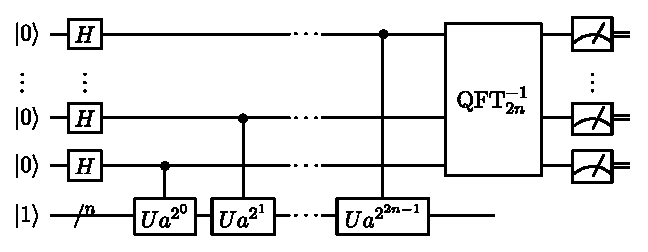
\includegraphics[width=12cm]{pic/Shor_algorithm.eps}
\caption{Circuit of Shor's algorithm}
\label{ShorAlgorithm}
\end{figure}

\subsection{Complexity}

\section{Phase estimate and quantum Fourier transform}

\begin{equation}
\begin{array}{rl}
\keta{s_k} &= \frac 1 {\sqrt{2}} ({\keta{0}}_0+{\keta{1}}_0)
    \frac 1 {\sqrt{2}} ({\keta{0}}_1+e^{\frac {k*2 \pi i} 2}{\keta{1}}_1)
    ...  \frac 1 {\sqrt{2}} ({\keta{0}}_{n-1}+e^{\frac {(n-1)*2\pi i} 2^(n-1)}{\keta{1}}_{n-1}) \\
    ... \\
    &= \frac 1 {\sqrt{N}} \prod^{n-1}_{l=0} ({\keta{0}}_l+e^{\frac {k\times l \times 2\pi i} 2^l}{\keta{1}}_l) where k=0, 1, ...N-1.
\end{array}
\end{equation}
Like the $\keta{+}$ and $\keta{-}$ waves, each of the $\{\keta{s_k}, k=0, 1, ... N-1\}$ waves is a mixture of all the base waves, but they have different orientations in the $N$ dimension Hilbert space.


\chapter{Search algorithms}
\section{Grover's algorithm}
Like the Deutsch's algorithm, the Grover's algorithm also assumes a blackbox function $f(x)$ whose variable $x$ is a $n$-bit binary variable while its result is almost always 1 except at a few unknown points $x=x_w$. We assume $f(x_w)=-1$ at these exceptions. The goal of the algorithm is to find the $x_w$. Lov Grover proposed in 1996 that quantum computer can solve it faster than conventional computers.

To illustrate the algorithm, assume there is one and only one $x_w$ which is the search solution. Let's note $x_w$ in binary as $w_{n-1}...w_i...w_1 w_0$ where $w_i = 0 or 1$,
and $\Vec{w} = (0, 0, ..., 1 at i=w, ..., 0)^T$ as a $2^n-1$ dimensional vector.

Using conventional computers, the naive algorithm is to feed the $2^n -1$ possible numbers of $x_w$ one at a time to $f$ to test whether the result equals $-1$. It is a brute force algorithm. The worst case is that we have to do $2^n-1$ evaluations of $f(x)$ to find out $x_w$.

The desired best case is to explore all the possible $x_w$ at the same time. We naturally choose $\vec{S} = \frac 1 {\sqrt{2^n}} (1, 1, ...1)^T$, which is the sum of all the basis of the qubits, to feed the oracle function $f$.

We know, $\vec{S} = \vec{S} - \frac 1 {\sqrt{2^n}} \vec{w}) + \frac 1  {\sqrt{2^n}} \vec{w}$. Apparently, $\vec{S_1}  = \vec{S} - \frac 1 {\sqrt{2^n}} \vec{w}$ is a vector orthogonal to $\vec{w}$, and applying the $F$ gate to it does not change its phase. Therefore, $F(\vec{S}) = F(\vec{S_1}) + F(\frac 1  {\sqrt{2^n}} \vec{w})  = \vec{S_1} - \frac 1 {\sqrt{2^n}} \vec{w}$. We see that 
\begin{itemize}
    \item applying the $F$ gate turns vector $\vec{S}$ toward $-\vec{w}$
    \item applying the $F$ gate to $\vec{S_1}$ makes no change.
\end{itemize}
Therefore, can we apply $F$ gate $2^n$ times and turn $\vec{S}$ completely to $-\vec{w}$? But applying $F$ gate once more will change the phase of the $\vec{w}$ vector back. We need to change the sign of vector $\vec{w}$ first while preserving its angle with $\vec{S}$ before applying $F$ gate again. This can be accomplished by apply gate $U_S = 2 \vec{S}X\vec{S} -I$, which flip $\vec{w}$ around the vector $\vec{S}$. However, when implementing this flip, we need to rotate $vec{S}$ to the $\vec{0}$, do the flip, and rotate the frame back to $\vec{S}$.

\begin{figure}[h]\label{Grover}

\caption{Applying F gate}
\end{figure}

\subsection{Complexity}

\section{Simon's algorithm}
The Simon's algorithm assumes a blackbox oracle function $f(x)$ whose variable $x$ is a $n$-bit binary variable. Its results are $m$-bit values that are periodic, but the period $t$ is unknown -- $f(x+t)=(fx)$ for all $x$. How do we find the period $t$? Of course, we are tempted to play the trick again of feeding $\vec{S} = \frac 1 {\sqrt{2^n}} (1, 1, ...1)^T$ to the oracle function $f$. We have
$f(\vec{S}) = \frac 1  {\sqrt{2^n}} \sum_x f(x)$.

\subsection{Circuit diagram}
\begin{figure}[h]
\begin{quantikz}%[slice all, slice style={shorten <=8mm}, slice label style = {yshift=-38mm} ]
    & & &\lstick{Alice' 2nd bit}  & \cwbend{2} \\
    & & \lstick{1st bit}  & \cwbend{1} \\
    \lstick{\ket{0}} & \gate{H} &\ctrl{1} & \gate{Z} & \gate{X} &\ctrl{1} & \gate{H} & \meter{} &\cw \rstick{Bob's 1st bit} \\
    \lstick{\ket{0}} & \qw      & \targ{} \slice[style={shorten <=12mm}, label style={yshift=-38mm}]{BS1} & \qw \slice[style={shorten <=12mm}, label style={yshift=-38mm}]{BS2} & \qw \slice[style={shorten <=12mm}, label style={yshift=-38mm}]{BS3} & \targ{} & \qw & \meter{} & \cw \rstick{Bob's 2nd bit}
\end{quantikz}
\caption{Simon's algorithm}
\label{Simon}
\end{figure}

\subsection{Complexity}
Using a conventional computer, finding the period takes $2^{n/2}$ operations.

\addcontentsline{toc}{chapter}{Appendix: Quantum Devices}
\chapter*{Appendix: Quantum Devices}\label{A-qubit}
\section{Types of waves}
Communication requires waves to propagate from one place to a remote place. Quantum computer qubits require stationary waves. By propagation characteristic, we can differentiate waves into propagating waves, standing waves and trapped waves.

Radio-frequency (RF) electromagnetic waves are used for mobile communications including Wi-Fi. They can spread everywhere unless blocked or confined by reflective matters. Light waves -- electromagnetic waves with wavelength ranging from sub-micron to a few microns -- are used for optical communications. They can be channeled by optical waveguides such as optical fibers to explore different paths. They are confined in two dimensions -- the lateral dimensions -- but propagate in axial dimension along the the waveguides or fibers. Propagating waves are not ideal for building qubits for quantum computing. However, there have been clever designs that construct quantum computing circuits entirely using integrated optical waveguides.

If an electromagnetic wave is confined in three dimensions, such as in a microwave oven, the wave cannot propagate anywhere other than being reflected back and forth within the confinement. And only standing waves of specific frequencies can exist. The allowed frequencies are discrete. Standing waves are good for storing information. Superconductor qubits are constructed using standing waves of electrons, as described below. Standing waves may be best visualized and understood through the vibration of a guitar string. When a string is plucked, the propagation of the vibrations is stopped and reflected by the two fixed ends. Only the waves whose phases coincide after a complete round trip of reflection survive, while the other waves cancel each other out and are suppressed.

Another type of waves, which we may call trapped waves, is not confined by anything with boundaries but is instead trapped by forces extending to infinity. Electrons in an atom are trapped waves due to the electric force of the nucleus' positive charges. The waves extend to infinity but are concentrated within a nanometer around the nucleus. Trapped waves are also good for storing information. Trapped-ion and neutral-atom qubits are built by trapped electron waves.

\section{Devices using polarization modulation}
Polarization is the vibration direction of a wave. The polarization of an electromagnetic wave is perpendicular to its direction of propagation. An electron wave's spin may be considered its polarization and is measurable by applying a magnetic field. The angle of polarization $\theta$ can be used to represent information in addition to the wave's phase $\phi$. Many textbooks use electron spin qubits as examples. However, such type of qubits has not been adopted by practical experiments or products until recently\cite{nanotube} because of the difficulty of building spin-manipulating devices.

Physicists have studied polarization of lights for hundreds of years. Engineers have developed all sorts of polarization-manipulating devices. Combination of polarization and phase modulation has been widely used in communication. The dominating modulation for free-space communication and optical fiber communication is dual polarization quadrature phase shift keying (DP-QPSK). Free space communication is mostly used for satellite-satellite communication. There is no substance in space to degrade the power of light waves. Free space communication can also be used for ship-ship and building-building communication on earth if the distance is not too far. Optical fiber communication is the fastest and cheapest choice for any wired communication of distance 100 meters or longer. The dominant modulation for long-distance optical fiber communication is also DP-QPSK.

Qubits for optical quantum communication naturally use the combination of polarization and phase modulation. Optical qubits have also been demonstrated in laboratories for quantum computing. Gates require manipulating wave polarization. They use optically transparent birefringent materials that have different speeds for lights of different polarization. Placing such a material in a light generator e.g. a laser, generation of light in one polarization direction is favored while the others are suppressed. A half-wave plate made from such a crystal can change the polarization angle of a light to any direction. Fig. \ref{Polarization-splitter} is a type of prism that can split the horizontal and vertical polarization components of a light that has off-angle polarization.

\begin{figure}[h]
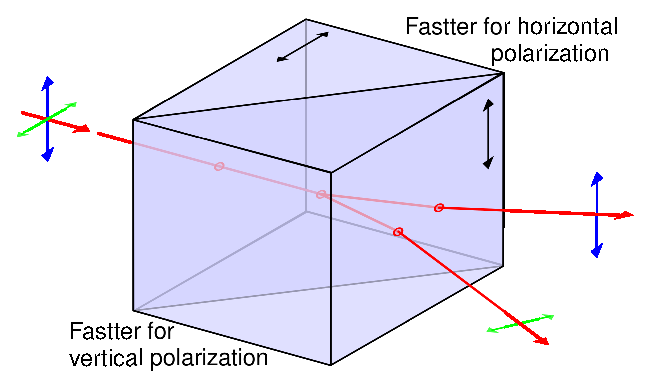
\includegraphics[width=10cm]{pic/polarization-prism.eps}
\caption{Polarization $cos{\theta} \keta{0} + e^{i \phi} sin{\theta} \keta{1}$}
\label{Polarization-splitter}
\end{figure}


\section{Devices using optical waveguides}
Waveguides confine waves in two dimensions and allowing them to propagate in once dimension. Optical fibers are the mostly deployed. A couple of decades ago, radio-frequency cables for broadcasting TV signals were mostly deployed.
Another type of qubits uses lights confined in optical waveguides. Optical fiber is a type of waveguide. We use the optical wave in the waveguide on the left in Fig. \ref{Fiber} to encode the binary number 0 and label it $\keta{0}$. We use the one in waveguide on the right to encode 1 and label it $\keta{1}$. The two waves have the same frequency and amplitude. They don't overlap and are of course orthogonal to each other. If we bring the two waveguides together to overlap (using an optical coupler), we get a superposition wave that is a sum of both waves. If the sum has $cos\theta$ amount in amplitude from $\keta{0}$ wave contributes and $sin\theta_p$ amount in amplitude from the $\keta{1}$ wave, we can use the value $\theta_p$ to characterize the superposition wave.

\begin{figure}[h]\label{Fiber}
%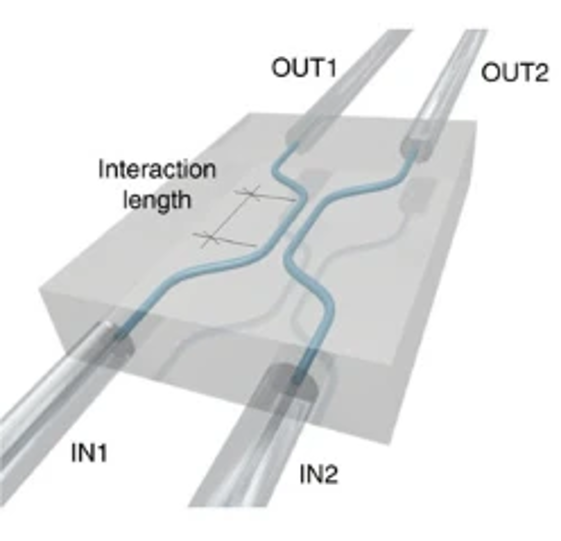
\includegraphics[width=6cm]{pic/wguideQubit.png}
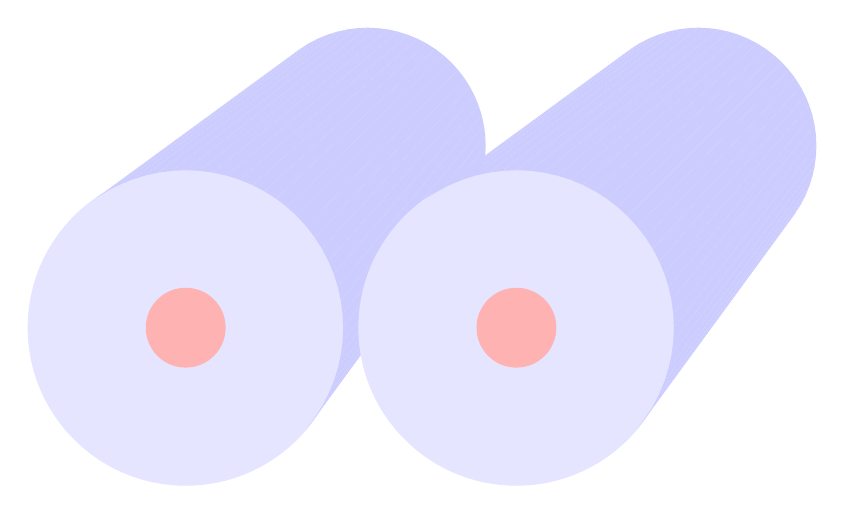
\begin{tikzpicture}[scale=0.5]
    \def\R{4} % Outer radius
    \def\Rb{3} % Outer radius
    \def\r{1} % Inner radius
    \def\L{6} % Half Length of the tube
    \def\S{4.2} % half Shift distance between tubes/fibers
    \def\I{5} % increment

    % Left tube
    \draw[blue!10,fill] (-\S,0,\L) circle (\R);   
    \draw[red!30,fill] (-\S,0,\L) circle (\r);    
    %\draw[decorate,decoration=zigzag] (-\S,0,-\L) circle (\Rb);
    \foreach \t in {-40,-35,...,123} {
        \fill[blue!20] ({\R*cos(\t+\I)-\S}, {\R*sin(\t+\I)}, \L) -- ({\R*cos(\t)-\S}, {\R*sin(\t)}, \L) 
        -- ({\Rb*cos(\t)-\S}, {\Rb*sin(\t)}, -\L) -- ({\Rb*cos(\t+\I)-\S}, {\Rb*sin(\t+\I)}, -\L) -- cycle;
    }

    % Right tube    
    \draw[blue!10,fill] (\S,0,\L) circle (\R);   
    \draw[red!30,fill] (\S,0,\L) circle (\r);    
    %\draw[black!10] (\S,0,-\L) circle (\Rb);
    \foreach \t in {-40,-35,...,123} {
        \fill[blue!20] ({\R*cos(\t+\I)+\S}, {\R*sin(\t+\I)}, \L) -- ({\R*cos(\t)+\S}, {\R*sin(\t)}, \L) 
        -- ({\Rb*cos(\t)+\S}, {\Rb*sin(\t)}, -\L) -- ({\Rb*cos(\t+\I)+\S}, {\Rb*sin(\t+\I)}, -\L) -- cycle;
    }
\end{tikzpicture}
\caption{A waveguide qubit comprised by two single-mode optical fibers $cos{\theta} \keta{0} + e^{i \phi} sin{\theta} \keta{1}$}
\end{figure}

The Xanadu.ai M-8 quantum computing chip assembles waveguide qubits and processing gates in an integrated waveguide circuit. We see it very much resembles a maze. The optical waveguides are the paths that light waves traverse. Its couplers and splitters resemble the junctions of maze. A coupler merge two light paths into one, and a splitter split one into two. The chip has 8 entrances and 8 exits and can build $8^8$ possible paths.

\section{Superconductor qubits}
A superconductor transmon qubit is similar to the string of a guitar and uses the first two standing waves, which resonate at the first and second harmonic frequencies respectively, to represent the integers of "0" and "1". Such a qubit is constructed by two superconductors separated by a layer of insulator. The insulator is thin enough for electrons to move ("tunnel") back and forth from one superconductor to another without loss of energy. But traveling through the insulator leads to delays (phase delays) of the electrons. The back-and-forth movement (vibration) of the electrons between the two superconductors resonate as standing waves at periods fractions of the delay. typically, the first fundamental frequency and the first harmonic are used to represent "0" and "1".
\begin{figure}[h]

\caption{Josephson junction}
\label{Superconductor}
\end{figure}

\begin{figure}[h]

\caption{Superconductor gates.}
\label{superGates}
\end{figure}

\section{Trapped atoms and ions}

\begin{figure}[h]

\caption{Atom}
\label{Atom}
\end{figure}

%\backmatter

\addcontentsline{toc}{chapter}{Bibliography}
\chapter*{Bibliography}
\bibliographystyle{unsrt}
   \bibliography{qcc}

\addcontentsline{toc}{chapter}{Index}
\printindex
\end{document}